\chapter{Introduction} \label{cpt-introduction}

Ever since the early days of computer graphics, both hard- and software have rapidly evolved
alongside the creative and challenging use cases provided by developers, scientists and others.
Many technical increments relied on innovation, especially the advent of new capable hardware.
One example is the \ac{GPU} itself, which is now considered the heart of modern graphics 
processing and is widely used in fields like science, artificial intelligence, games, and pretty 
much all graphics related applications. Before 1995, there already had been a lot of iterations 
on specialized graphics hardware, often focused on video formatting or color output operations
\cite{Singer2023}. [@TODO: Last sentence is redundant]\\

\noindent
The year 2024 marks the 25th anniversary of what is considered to be the first \ac{GPU}, the 
\emph{NVIDIA GeForce 256}. Although graphics chips had been around for a while, especially 
in the professional space of the industry, this card was the first to be marketed as a \ac{GPU}. 

\begin{quote}
    "\emph{What makes the GeForce different than its predecessors is the chip's ability to take over all 
    processing functions for creating three-dimensional graphics. Previously, the computer's main 
    processor would have to share in that responsibility, which could result in slower load times 
    and 'stuttering' on the part of the software.}" \\  
    (CNN Money \cite{CNNMoney1999}, 1999)
\end{quote}

\noindent
Before 1999, the graphics units were specialized chips either used for video encoding and decoding
or expensive hardware targeted for large companies, which arised during the early stages of "3D 
consumer graphics" \cite{Singer2023}. Dedicated and affordable \ac{GPU}s for consumer \ac{PC} had 
their large breakthrough during the 1990s. With the introduction of the \emph{NVIDIA GeForce 256}, 
efficient transformations and lighting computations found their way into private \ac{PC}s 
\cite{Fenno2024}. Back then, this new hardware created a multitude of new possibilities. Some of the 
major innovations featured \emph{cube mapping}, \emph{per-pixel light calculations}, and a 
\emph{standardized vertex buffer} \cite{NVIDIA1999, Battaglia2024}. [@TODO: Re-check vertex buffer] \\

\noindent
Although it was mostly used for graphics processing - hence the name - nowadays, \ac{GPU}s are used 
in a much more general way than in 1999. Both the technical complexity and the fields of application 
have tremendously increased. Today, a \ac{GPU} is often also referred to as a \ac{GPGPU} instead 
because of its evolution towards a multi-purpose tool. \\

\noindent
Nevertheless, \ac{GPU} architecture is still under a strong influence of the entertainment 
industry, first and foremost the games industry. Some of the latest changes to \ac{GPU} 
hardware and \ac{API} design correlates to the ongoing demand for higher output resolutions, 
higher geometric density or additionaly technology for \emph{Deep Learning} algorithms. 
These possibilities led to a lot more applications of \ac{GPU}s in various fields of science, 
like biology, machine learning, video encoding and decoding and more \cite{Battaglia2024}.
To provide more context for how we made use of some of the more modern features of \ac{GPU}s 
we will give a brief overview over the trends in computer graphics over the past decades, and 
especially the last years.


\section{Rise Of The GPU} \label{sec-rise-of-the-gpu}
[@TODO: Different chapter title (Historical development of the Rendering Pipeline)]
[@TODO: double check games]

\begin{figure}[h]
    \centering
    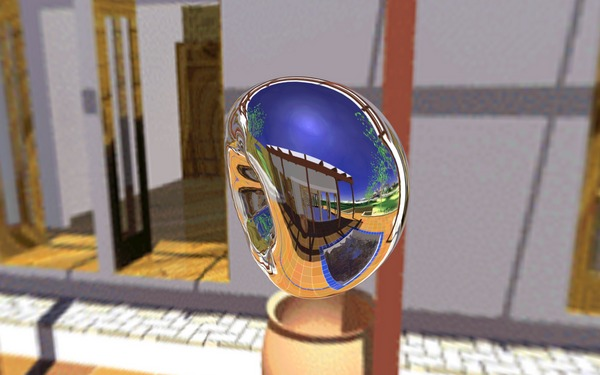
\includegraphics[width=250px]{images/graphics/bubble-reflection-effects-demo.jpg}
    \caption{The \emph{NVIDIA} bubble demo showcasing advanced reflections using cube mapping (\emph{NVIDIA} \cite{NVIDIABubble}, 2000).}
    \label{fig:bubble-reflection-demo}
\end{figure}

\noindent
Before the integration of specialized hardware, games like \emph{Wolfenstein 3D} or the 
original \emph{Doom} made heavy use of \ac{CPU} computations for graphics processing, 
executed sequentially \cite{NVIDIA1999}. A major problem was the demand for increasing 
geometrical detail. Games needed to get bigger, more photo-realistic and provide more dense 
geometry. Increasing the amount of triangles rendered, ultimately led to worse runtime 
performance. The advent of a dedicated, massively parallel chip to perform a large amount of 
operations introduced a solution for this problem. Over the years, more and more stages of the 
rendering pipeline were offloaded to the \ac{GPU}, which in turn resulted in a lot of new effects, 
games with higher triangle density and new lighting technology. As mentioned before, the \emph{NVIDIA 
GeForce 256} introduced cube mapping to the pipeline, featuring real-time reflections, which is 
shown in figure \ref{fig:bubble-reflection-demo} \cite{Battaglia2024}.


\subsection*{Rendering Pipeline} \label{subsec-rendering-pipeline}

The standardization of the graphics hardware, as pioneered by \emph{NVIDIA}, in concert with capable 
graphics \ac{API}s like \emph{Direct3D} or \emph{OpenGL} kick-started huge graphical improvements in 
games and computer graphics. The heavily parallelized transformations allowed for a lot more triangles 
in games, and the hardware accelerated lighting computations made for even more realistic lighting 
throughout the rendered scenes. One significant advantage: The \ac{GPU} could operate on a large amount 
of data while not stalling the \ac{CPU} \cite{Fenno2024}.\\

\noindent
The new rendering pipeline was to be seen in a lot of games, some of the first being \emph{Epic Games'} 
\emph{Unreal Turnament} (1999) and \emph{id Software's} \emph{Quake III Arena} (1999) \cite{UnrealTurnament, 
Quake3Arena}. \emph{Microsoft's} multimedia \ac{API} \emph{DirectX 7} added support for the new \ac{TL} 
features of \ac{GPU}s. During the following years, more and more features were added, slowly evolving the 
standard towards the "modern" rendering pipeline that is used nowadays. Between the years 1999 and 2009,
20 new minor versions of \emph{DirectX} were released \cite{WikiDirectX}. [@TODO: Check Wikipedia source] 

\begin{figure}[h]
    \centering
    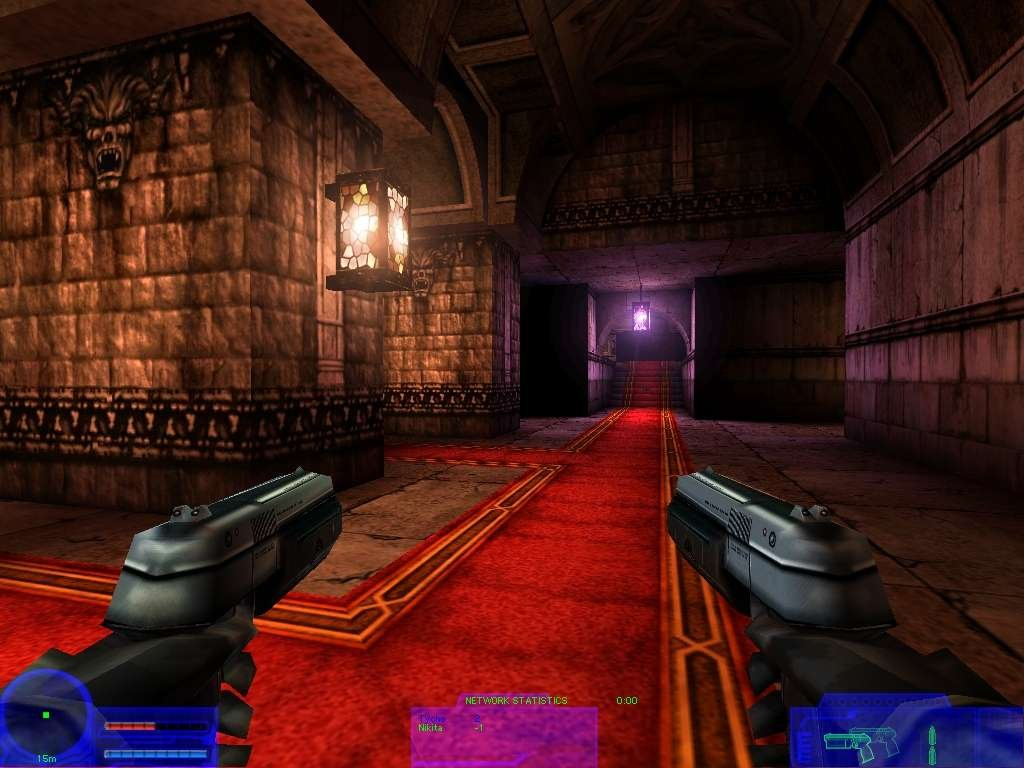
\includegraphics[width=172.5px]{images/graphics/unreal-turnament.jpg}
    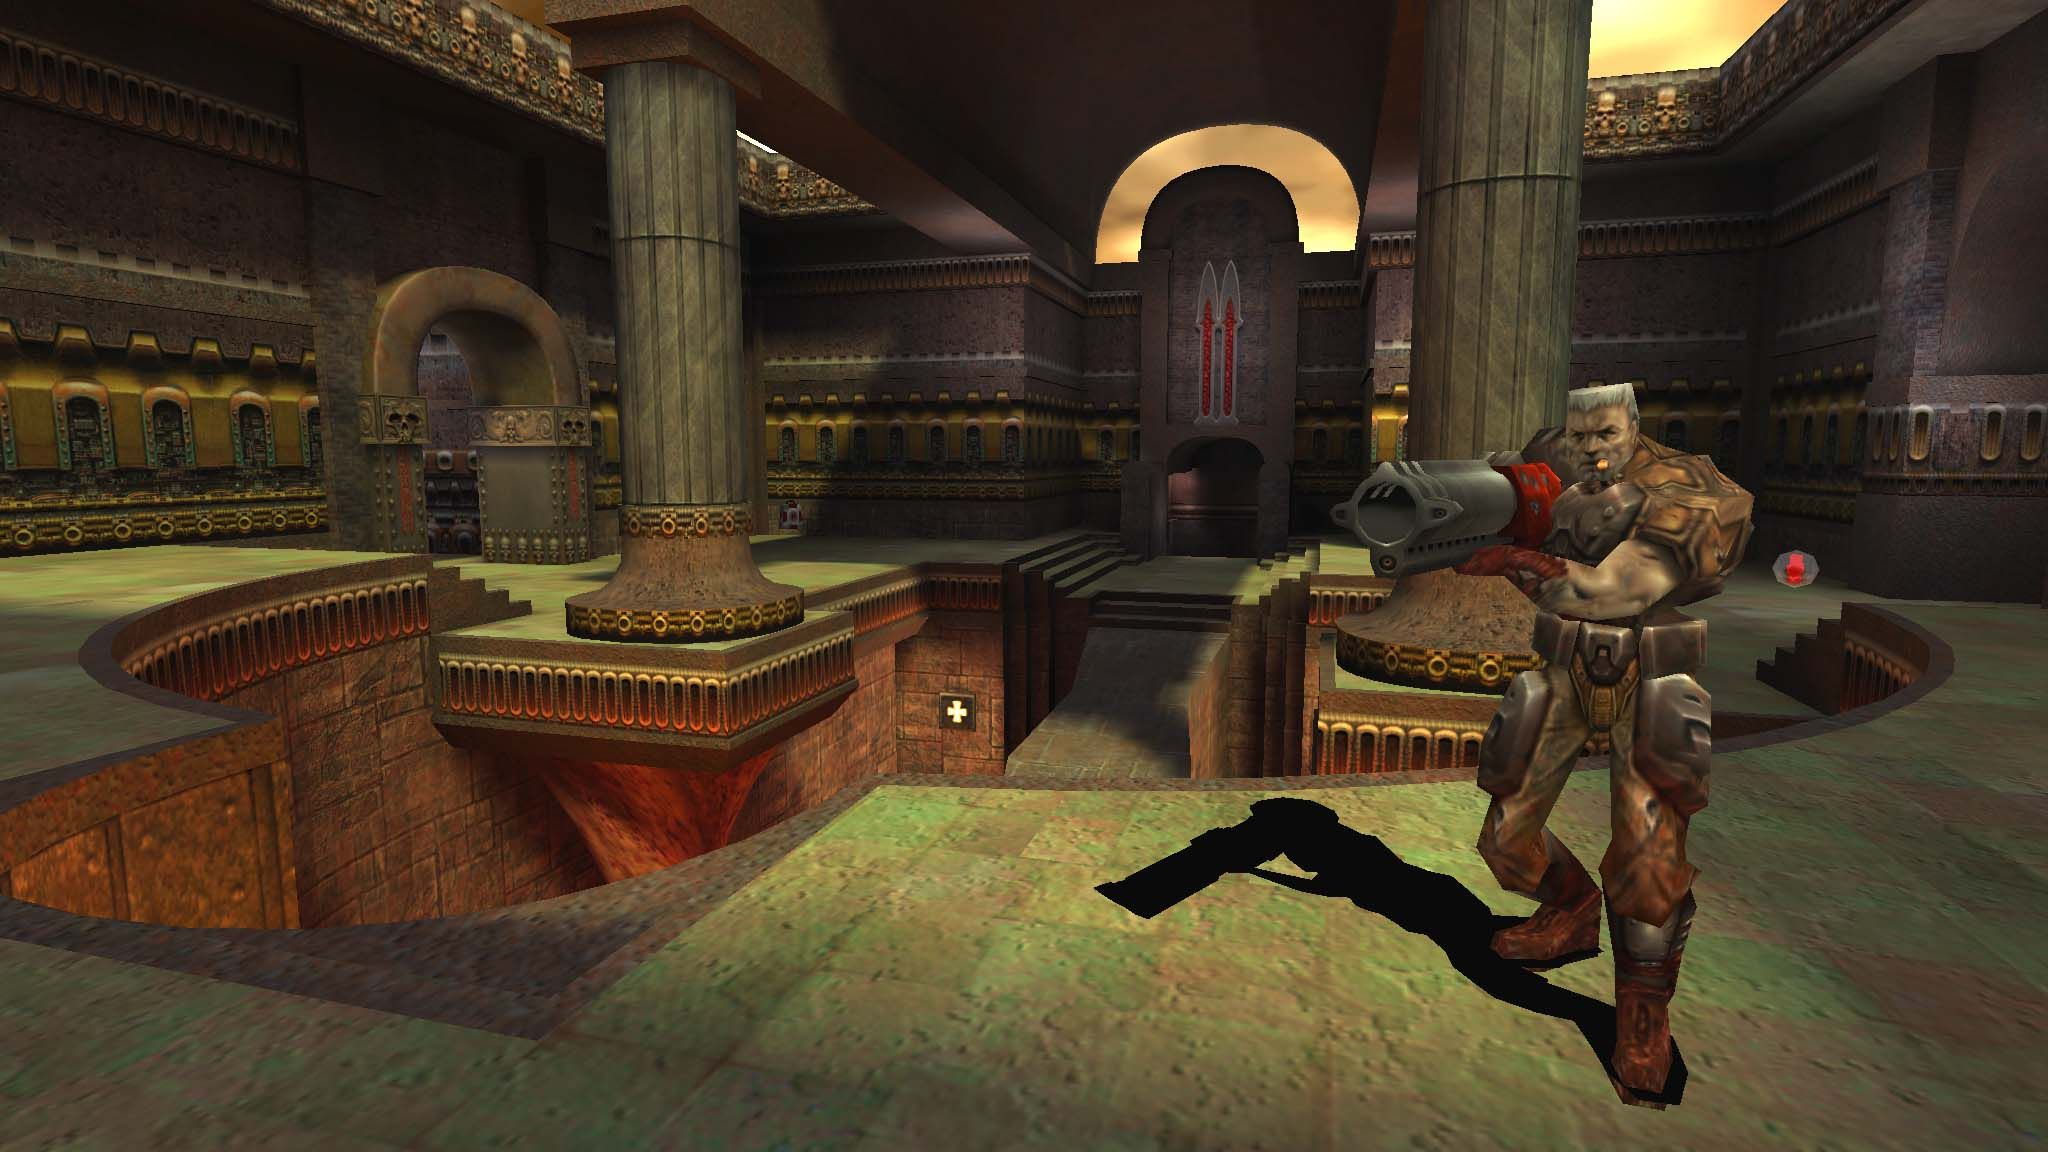
\includegraphics[width=230px]{images/graphics/quake-iii-arena.jpg}
    \caption{A screenshot from the game \emph{Unreal Turnament} (1999) (left) and \emph{Quake III Arena} (1999) 
    (right) \cite{GamespotUnrealTurnament, GameWatcher2006}.}
    \label{fig:unreal-turnament-quake-arena}
\end{figure}


\subsection*{Deferred Rendering} \label{subsec-deferred-rendering}

[@TODO: Sources]
With a lot of innovative hard and software, the games got complexer and real-time computer graphics got even more 
photo-realistic. The demand for more light sources increased in an attempt to make game worlds more realistic. 
However, more light sources posed some problems for the developers. When using the traditional rendering pipeline,
lighting is calculated on a per-vertex basis. Interpolation can be used to generate lighting results for every sample 
in between the vertices. Still, every vertex must be considered in combination with all light sources. This creates a 
dependancy between the amount of vertices and the amount of lightsources. Basically, adding a few more light sources 
will drastically increase computatoin times of the final image. Another method can be adopted: \emph{Deferred Shading}.
It was first adopted for the use on \ac{GPU}s by Dean Calver \cite{Calver2004} in 2004. This technique makes use of 
multiple render targets, and writes the data necessary for the lighting calculations into various buffers. This way, 
the surface normals, the specular intensity, the albedo (texture color), the depth and more values can all be stored 
individually, as per-pixel data. This includes the relevant data for the lighting calculations. When all buffers are 
drawn, the final result is easily found by looking up all the relevant data from each buffer at one pixel coordinate 
and combining them to a final result. Figure \ref{fig:deferred-shading-buffers} shows all the buffers used for the 
creation of one frame in \emph{Guerilla Games'} \emph{Killzone 2} (2007) \cite{KillzoneFandom}. 

\begin{figure}[h]
    \centering
    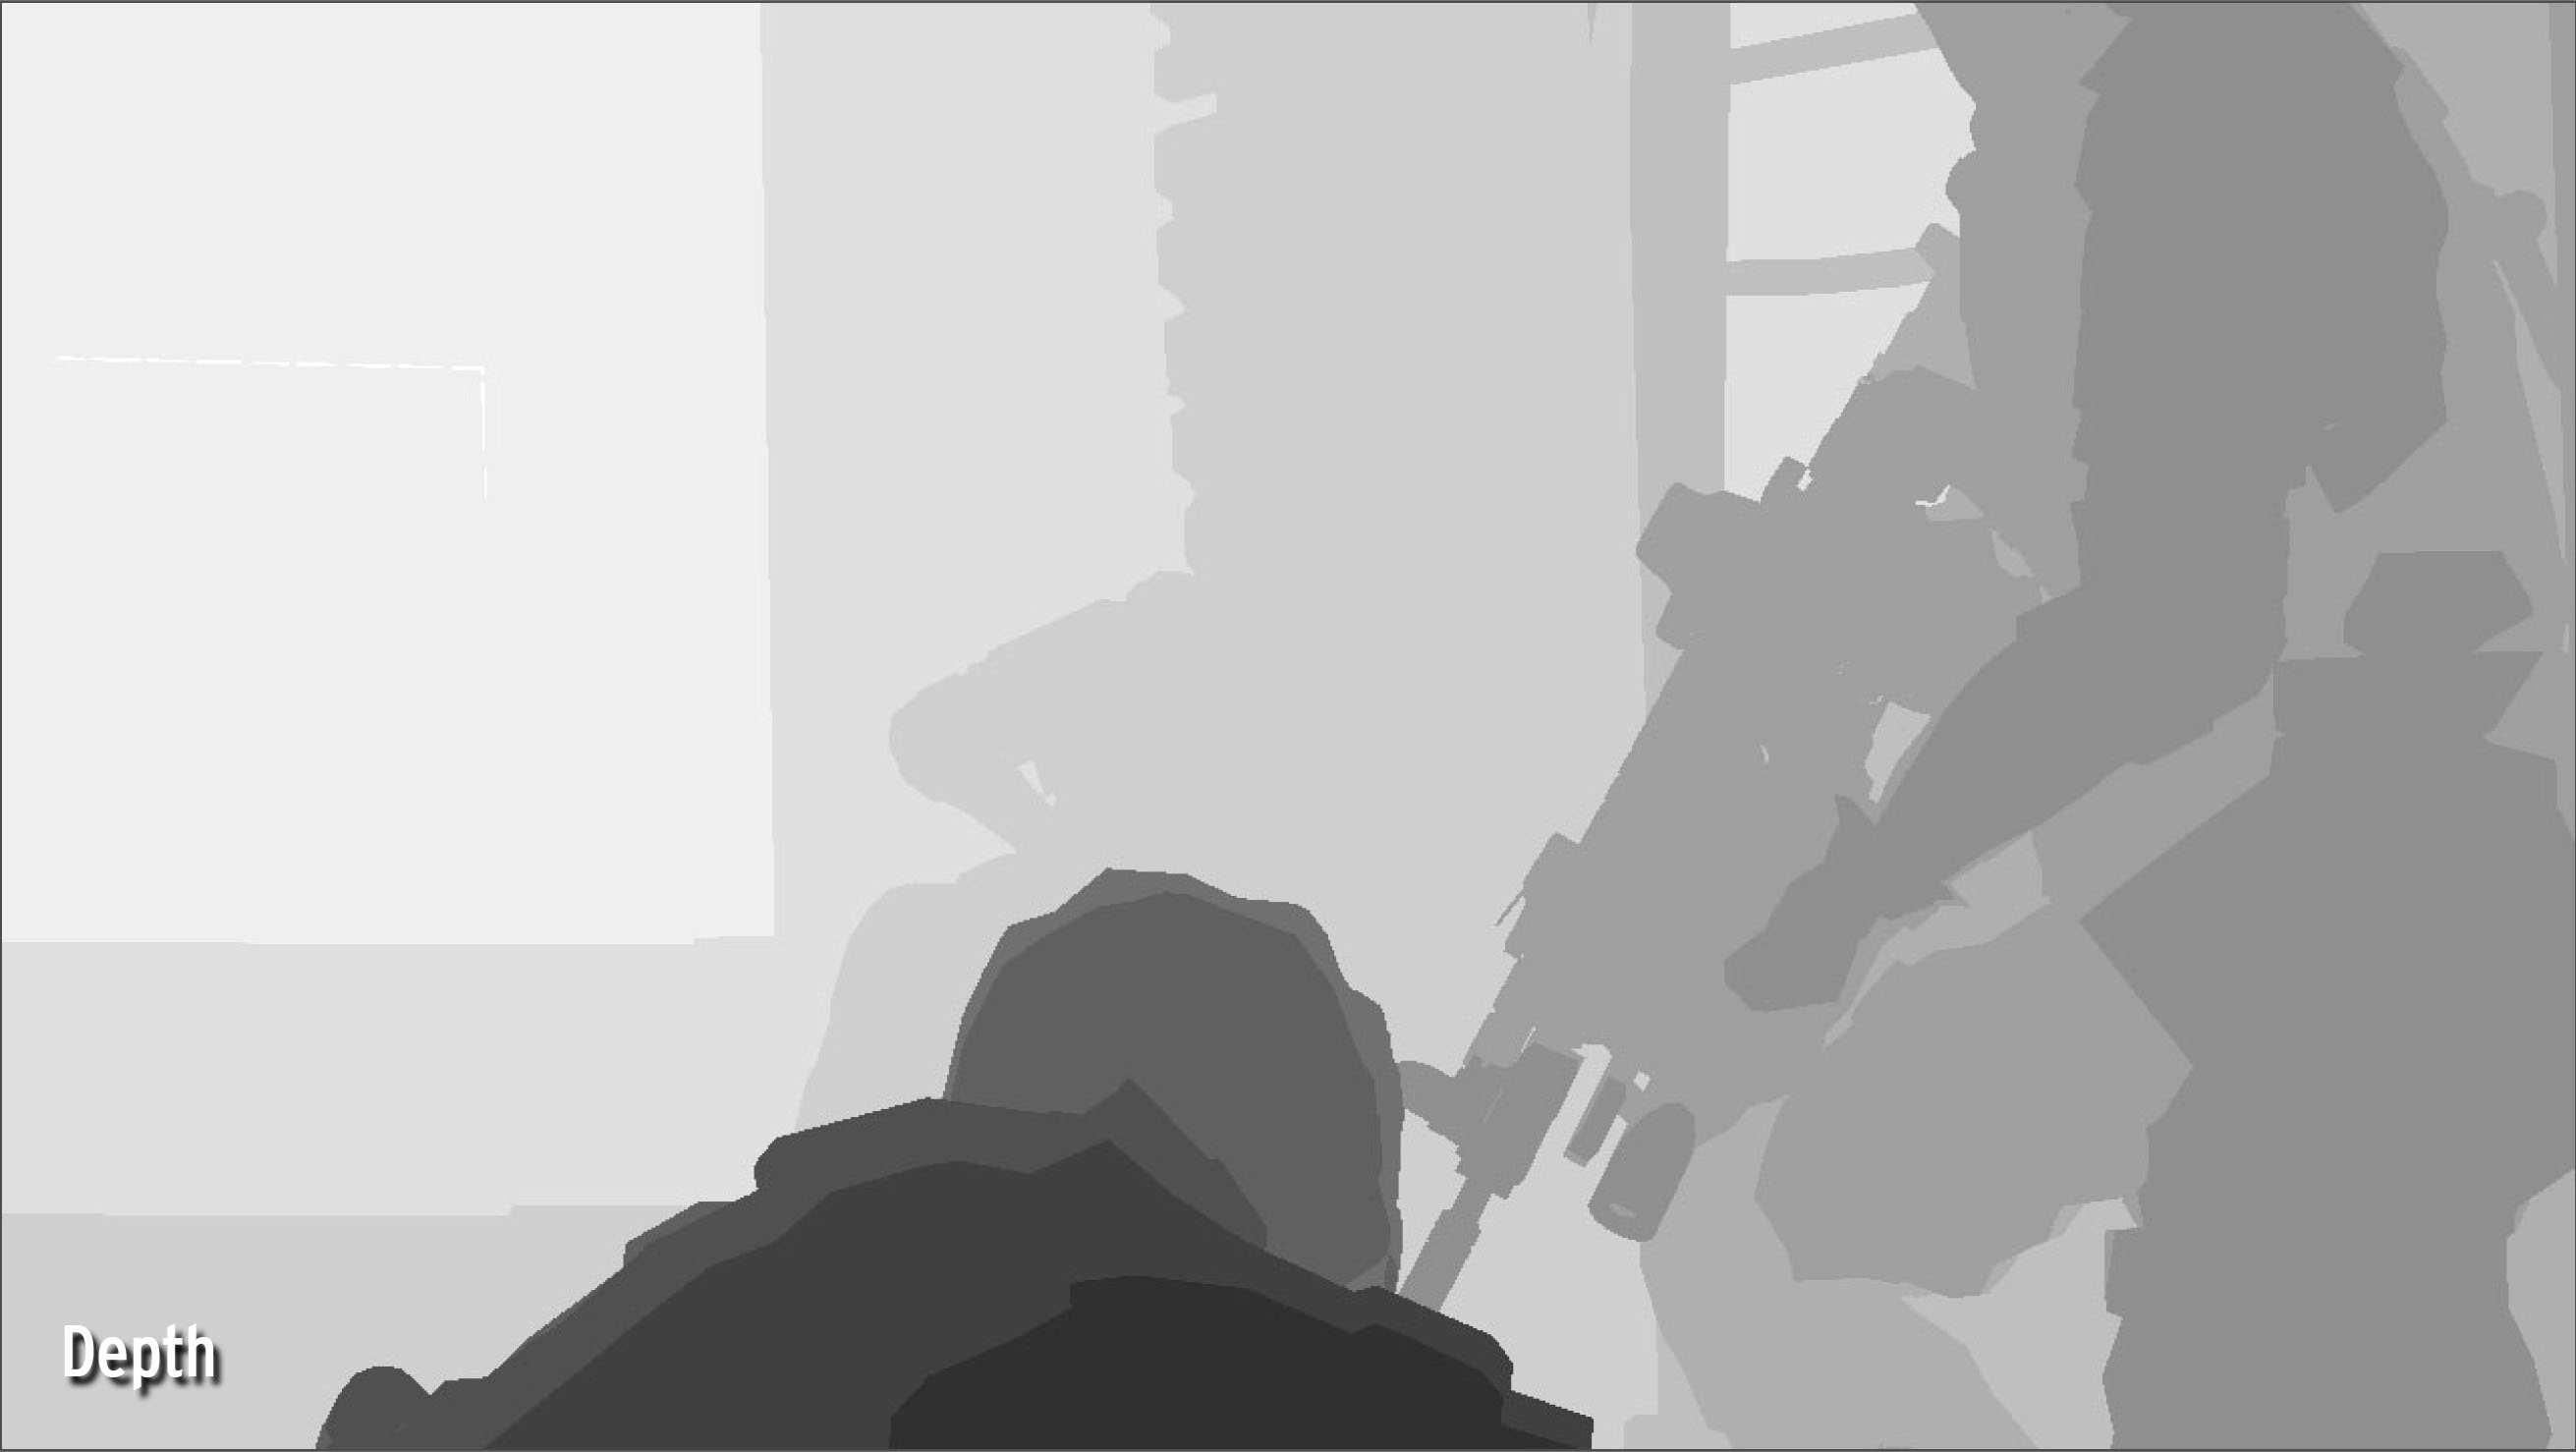
\includegraphics[width=175px]{images/graphics/killzone-2-buffer-depth.jpg}
    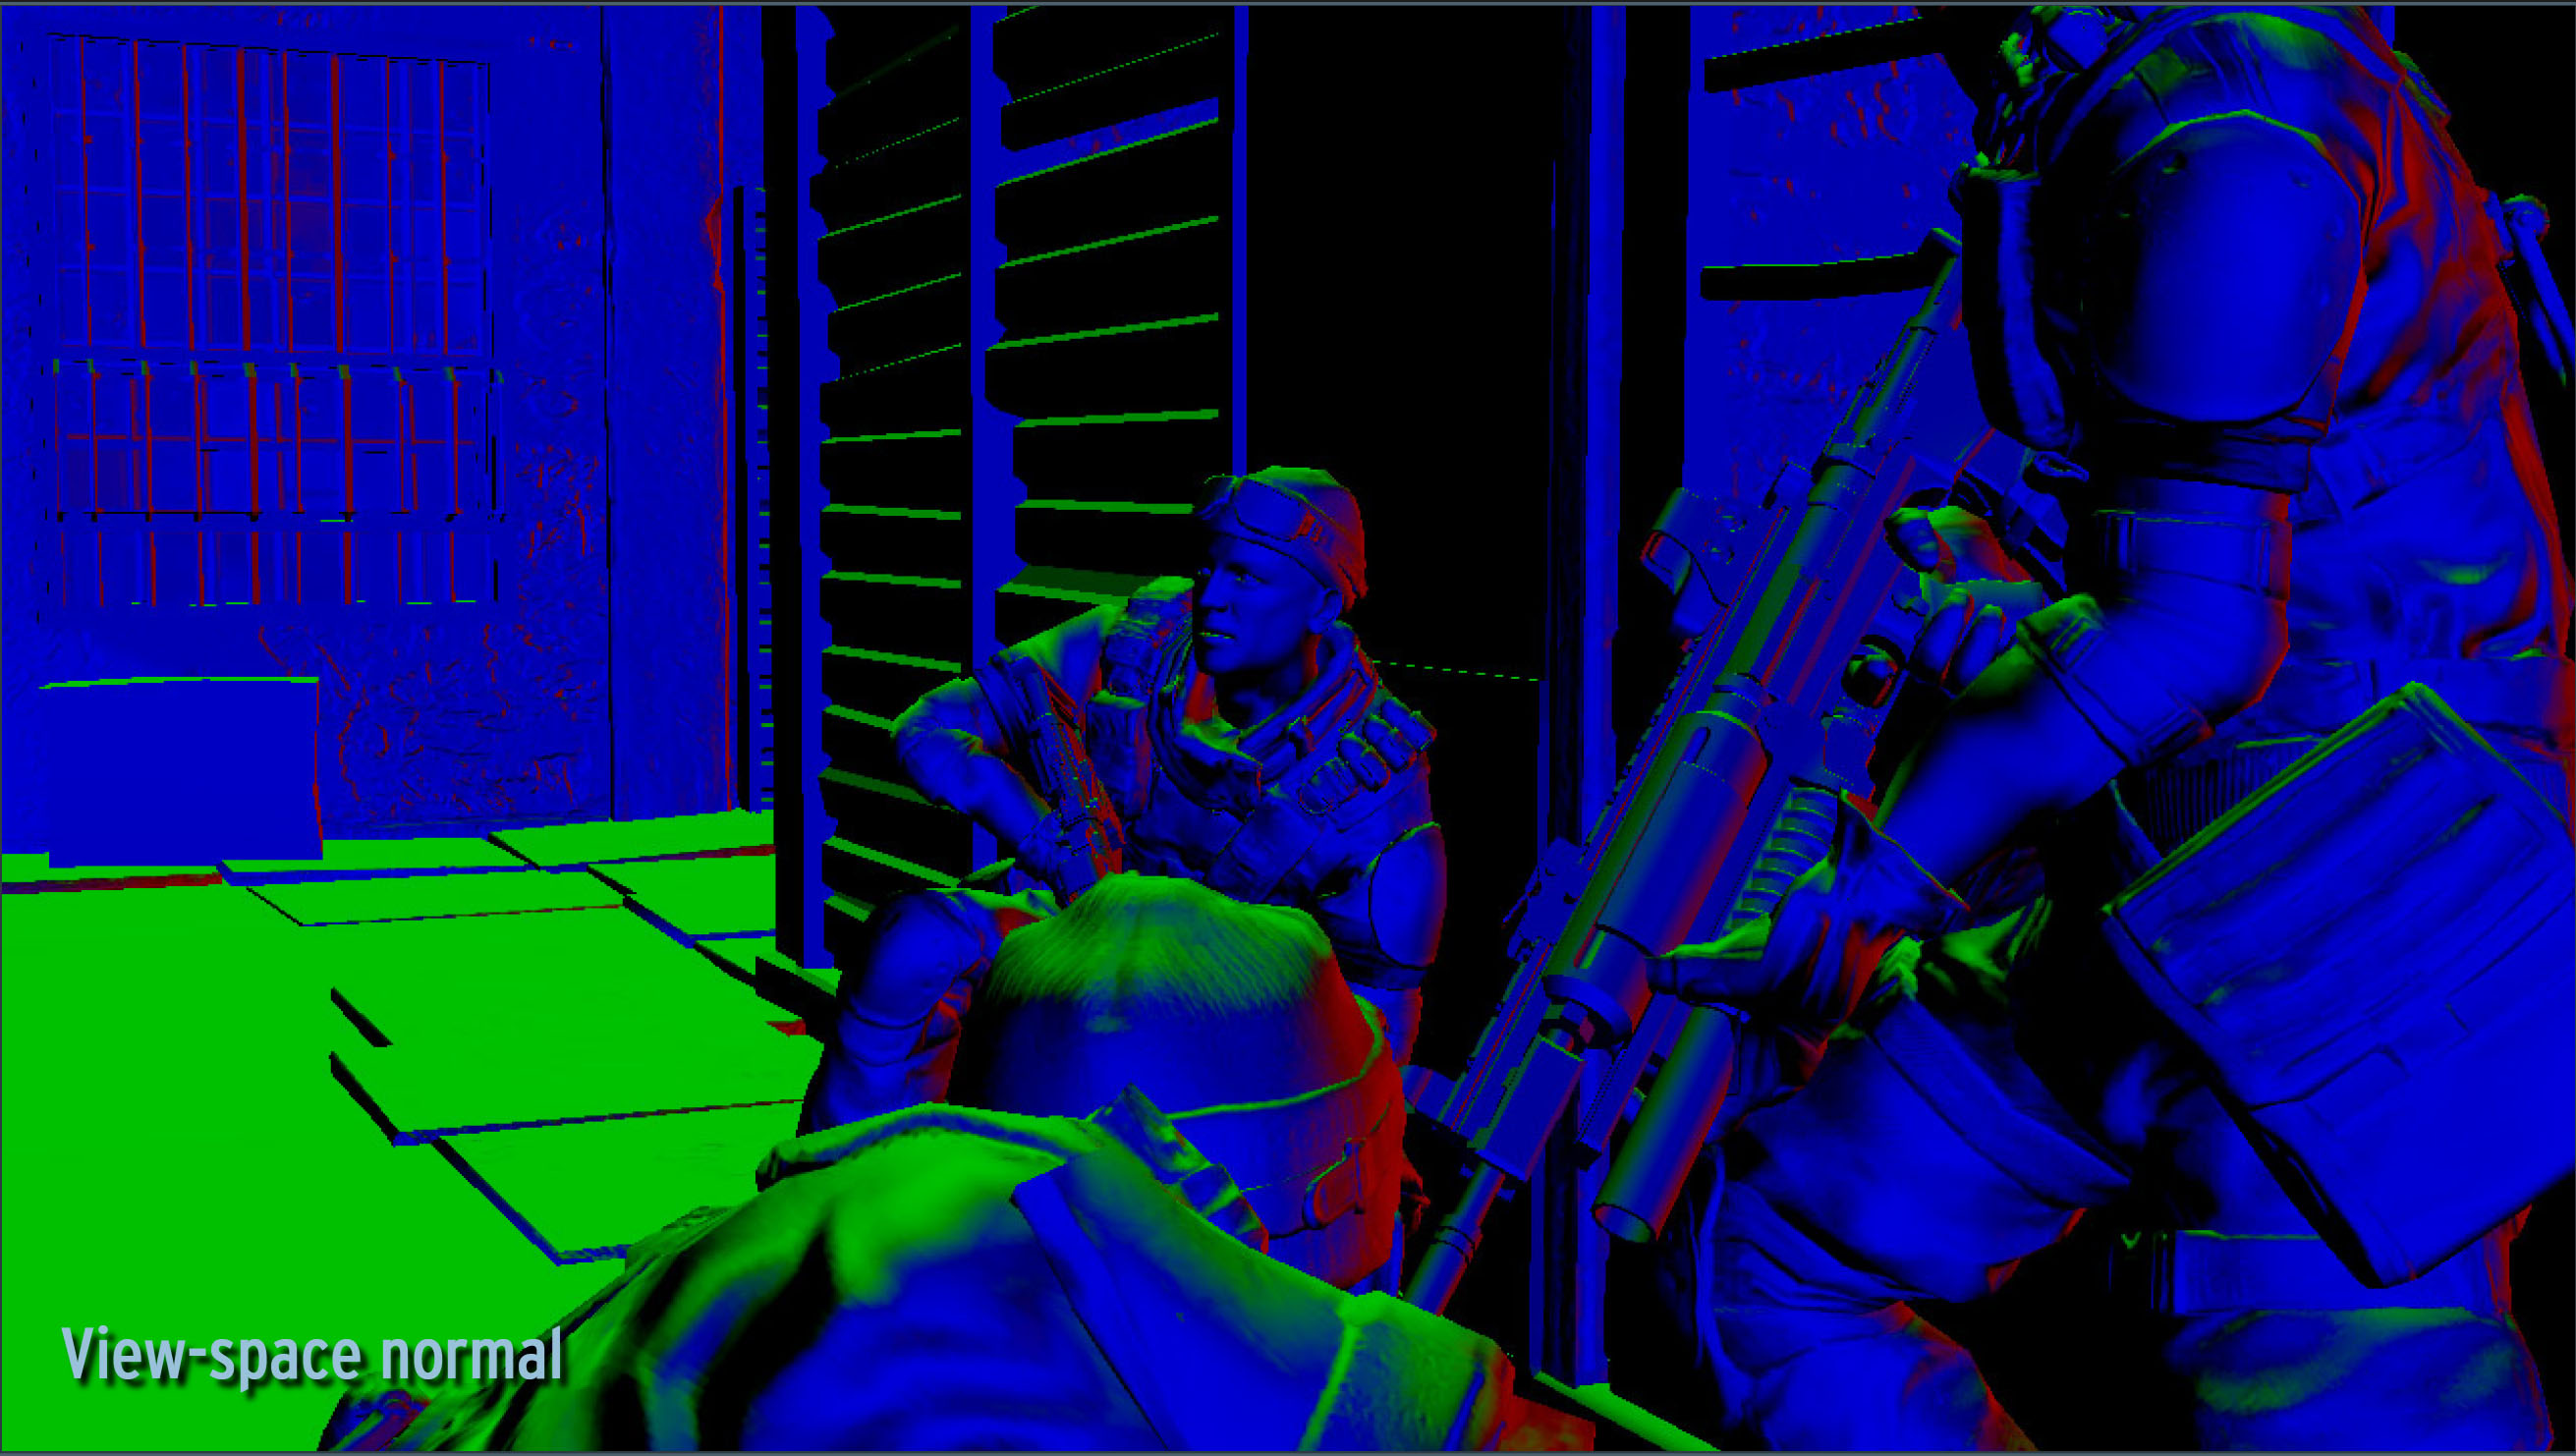
\includegraphics[width=175px]{images/graphics/killzone-2-buffer-vsn.jpg}
    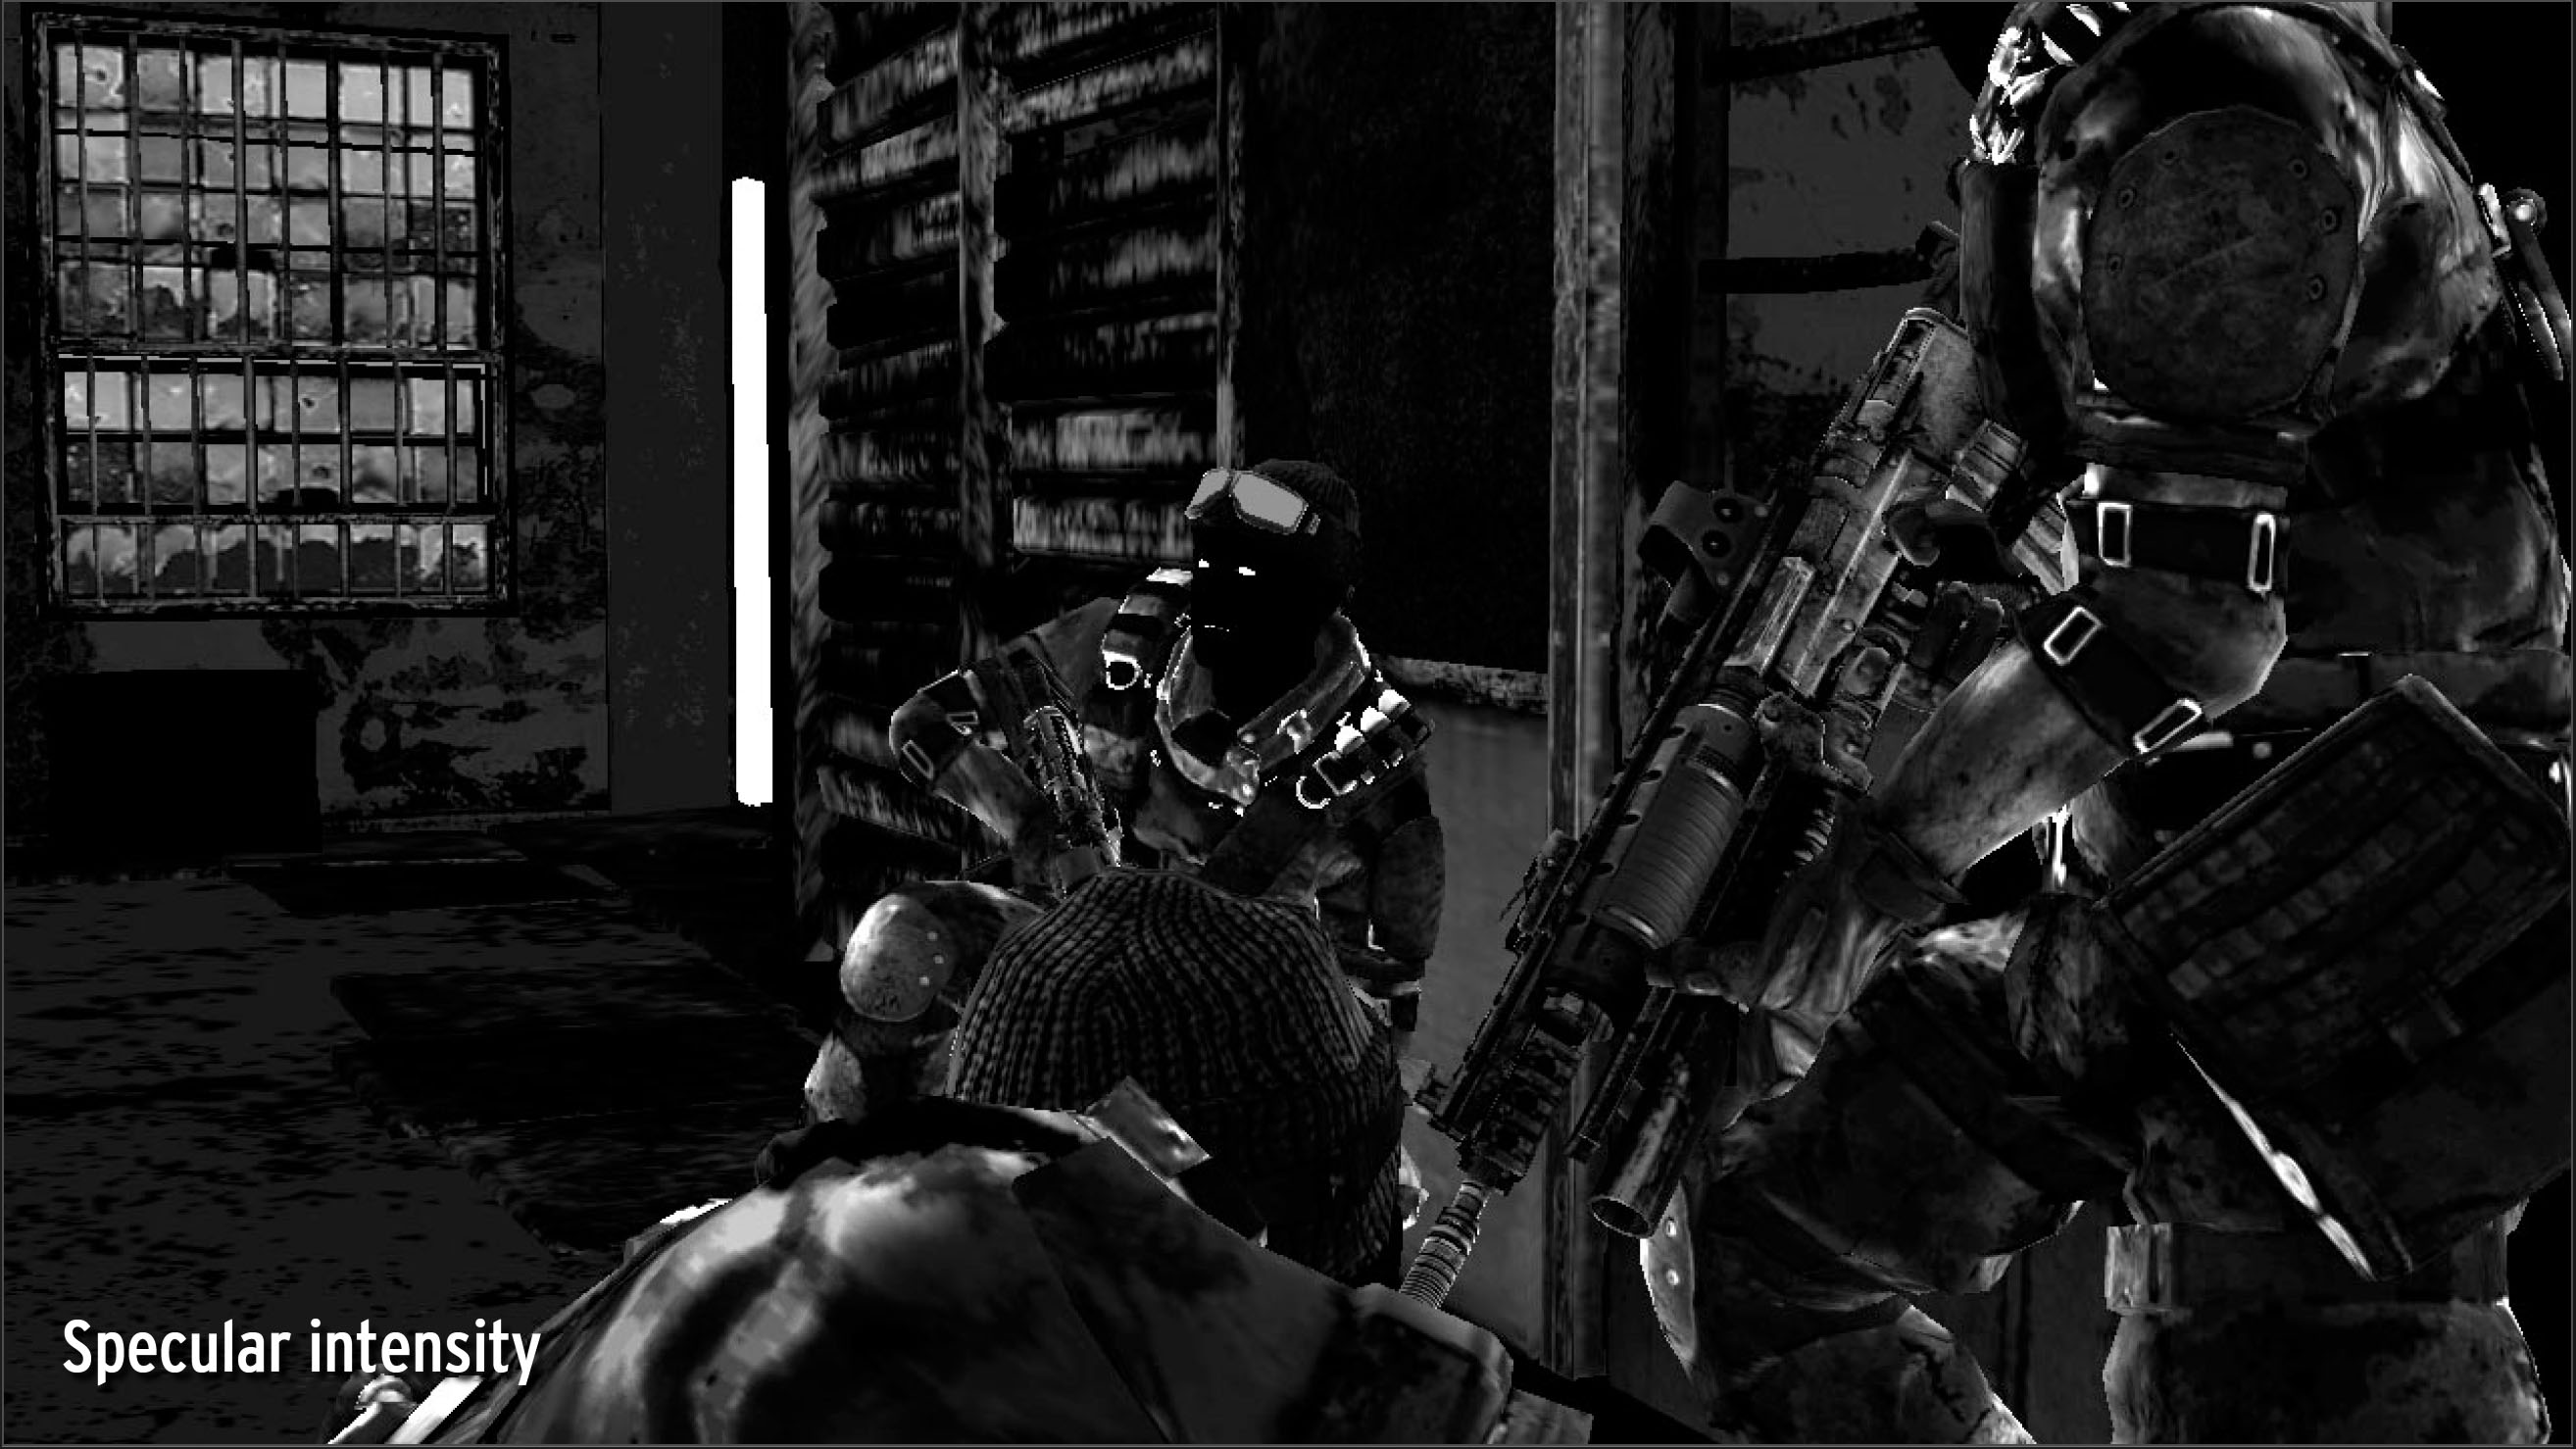
\includegraphics[width=175px]{images/graphics/killzone-2-buffer-specular.jpg}
    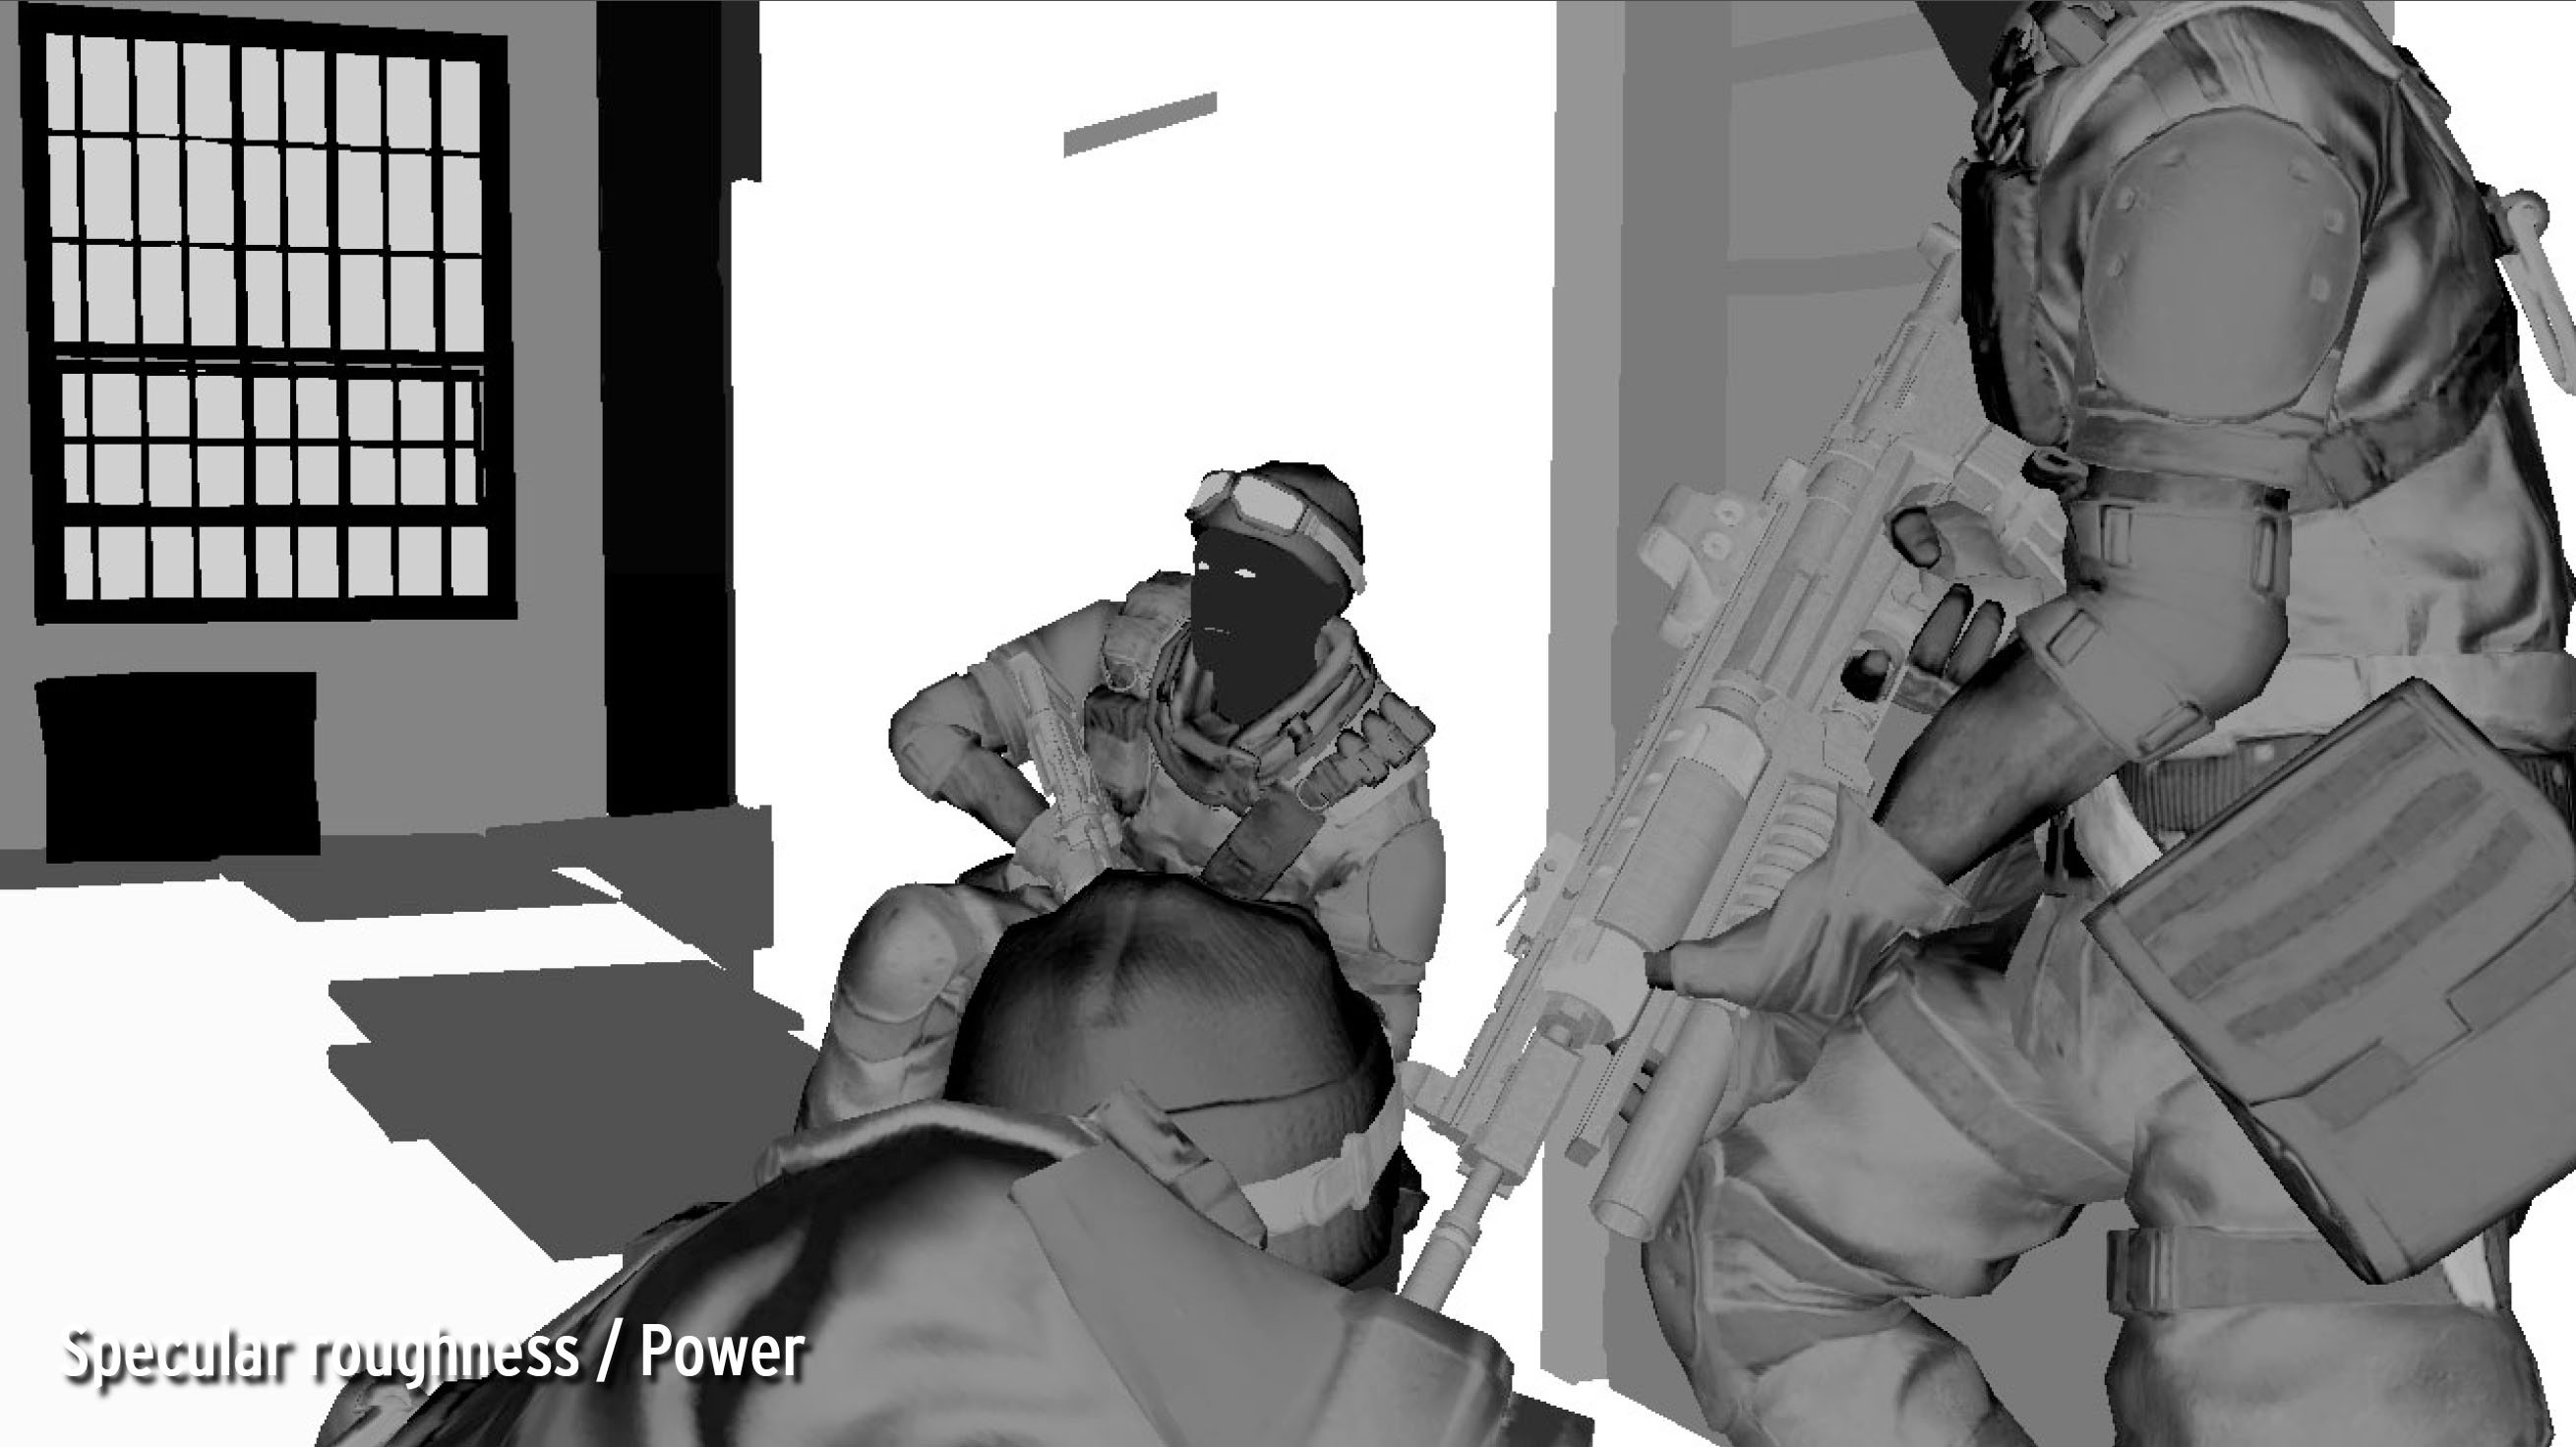
\includegraphics[width=175px]{images/graphics/killzone-2-buffer-specular-rough.jpg}
    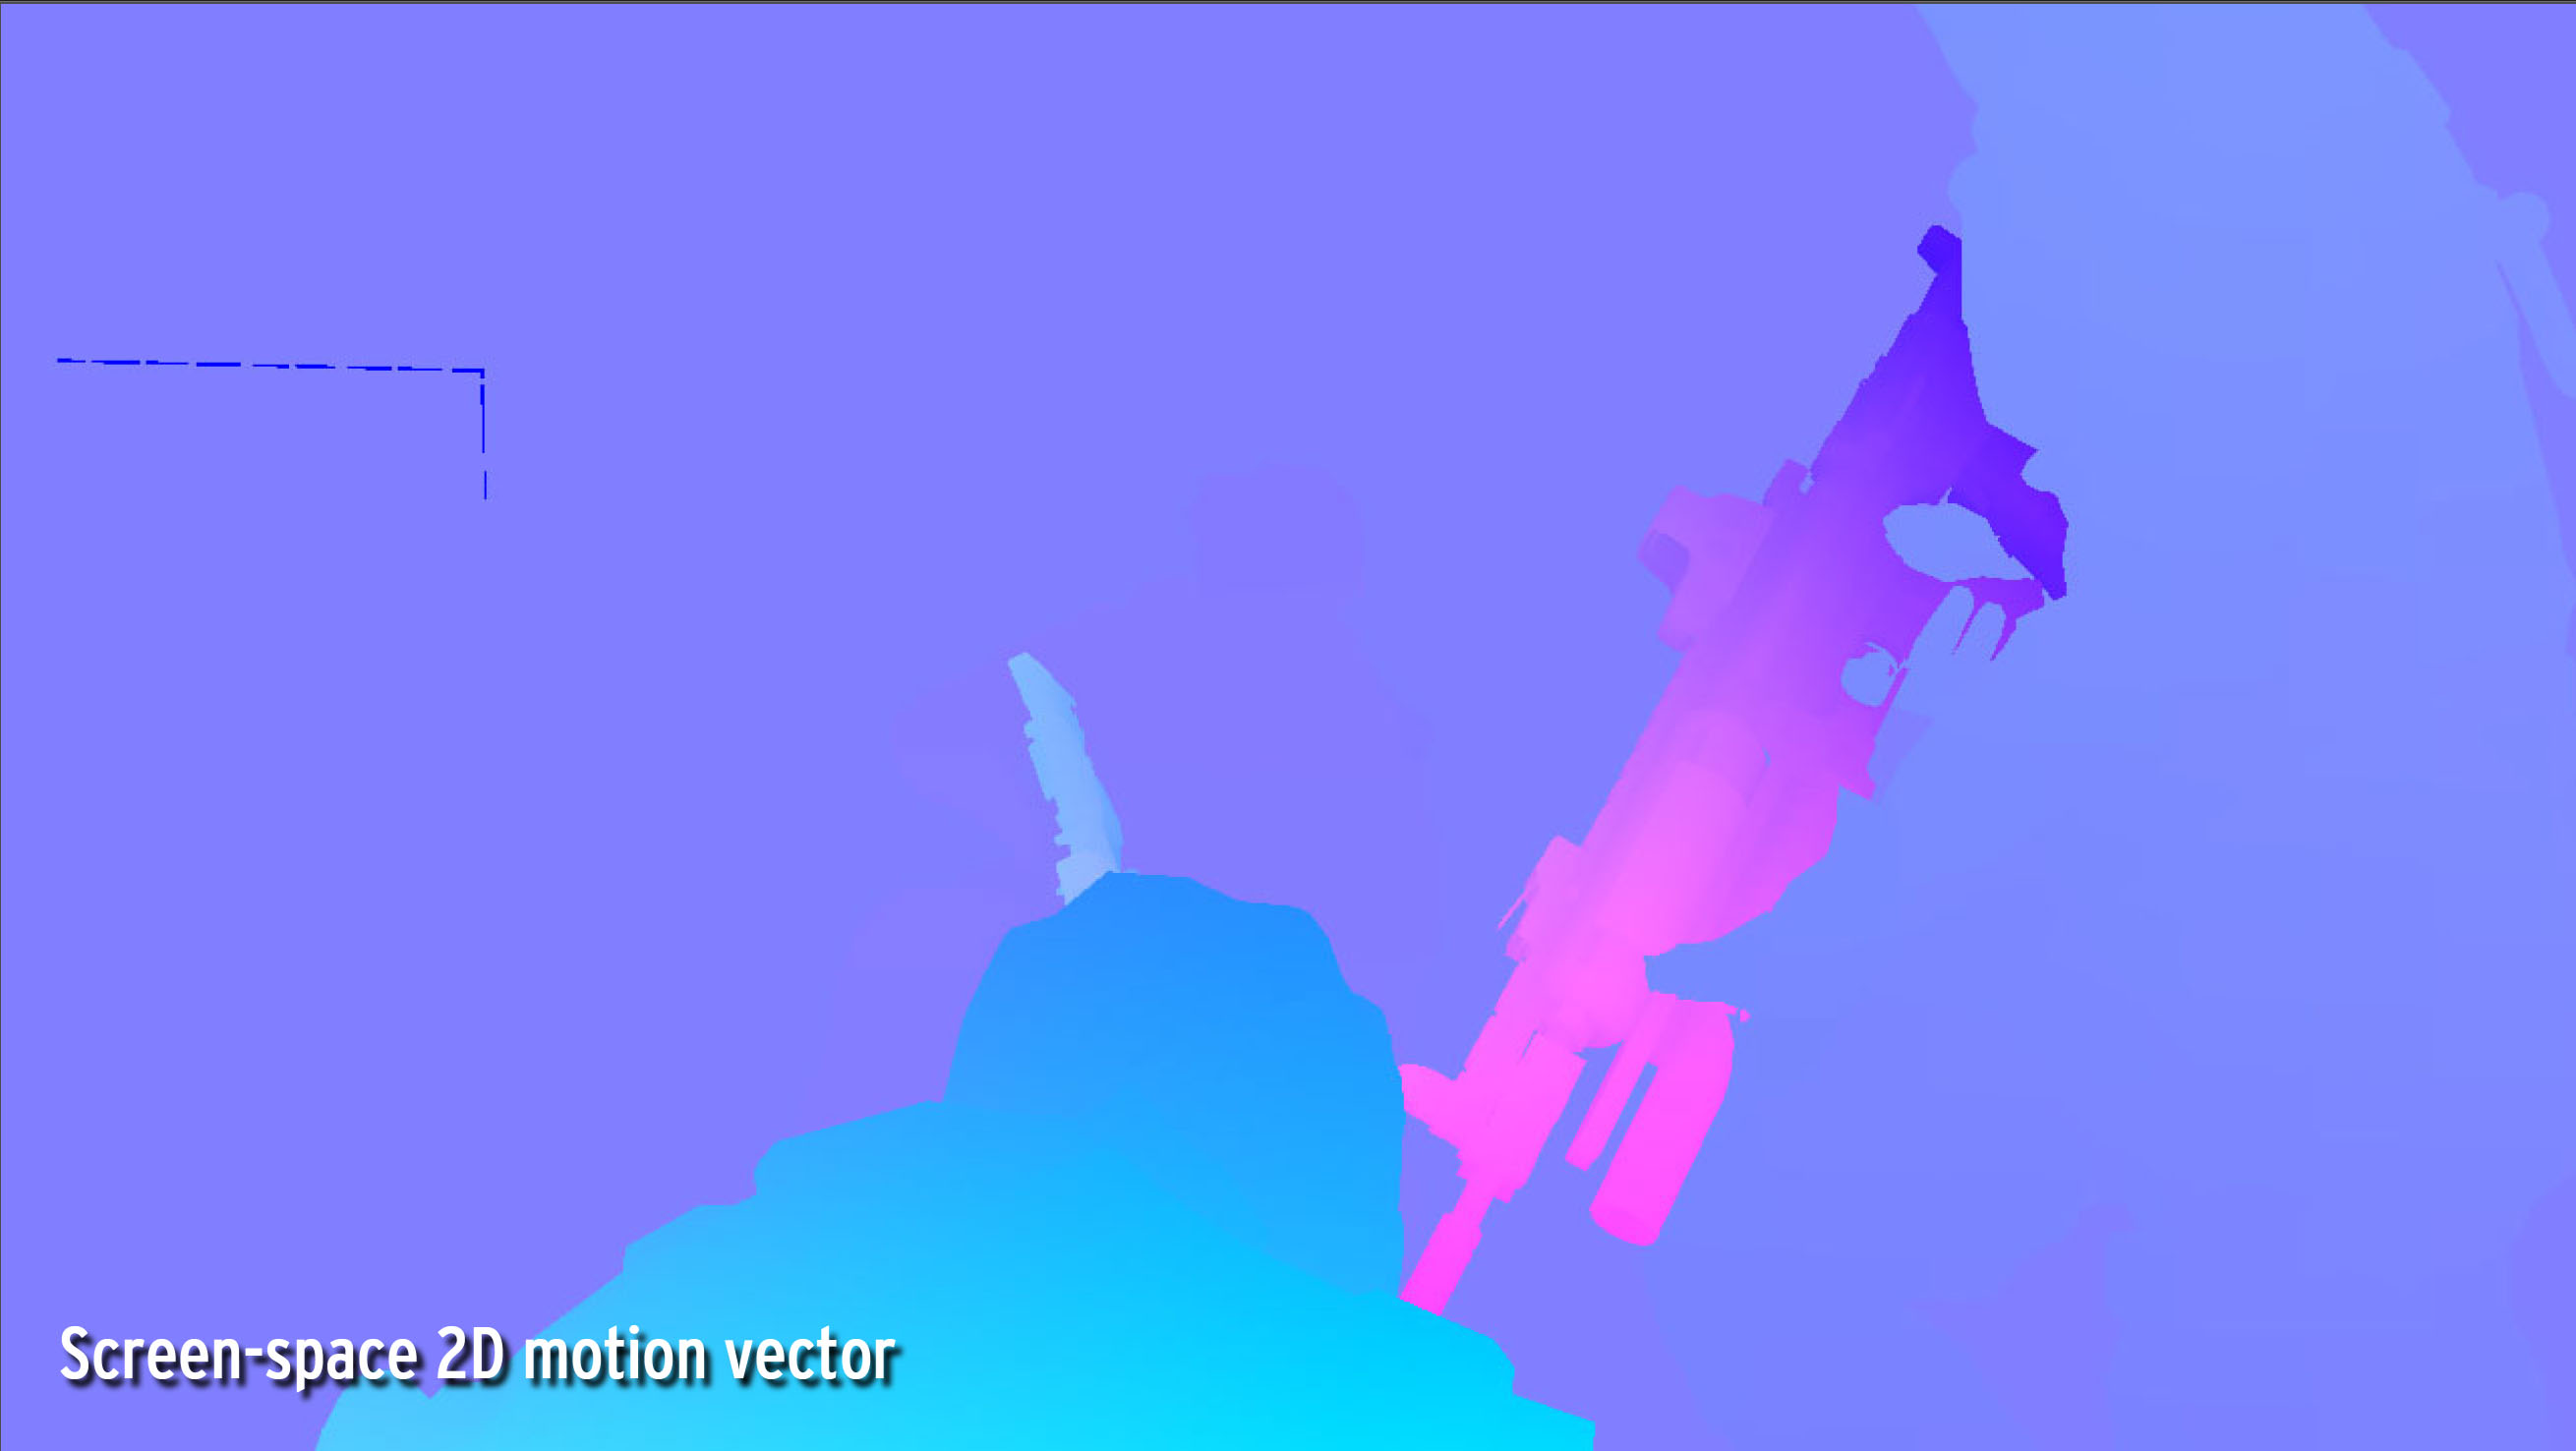
\includegraphics[width=175px]{images/graphics/killzone-2-buffer-ss-motion.jpg}
    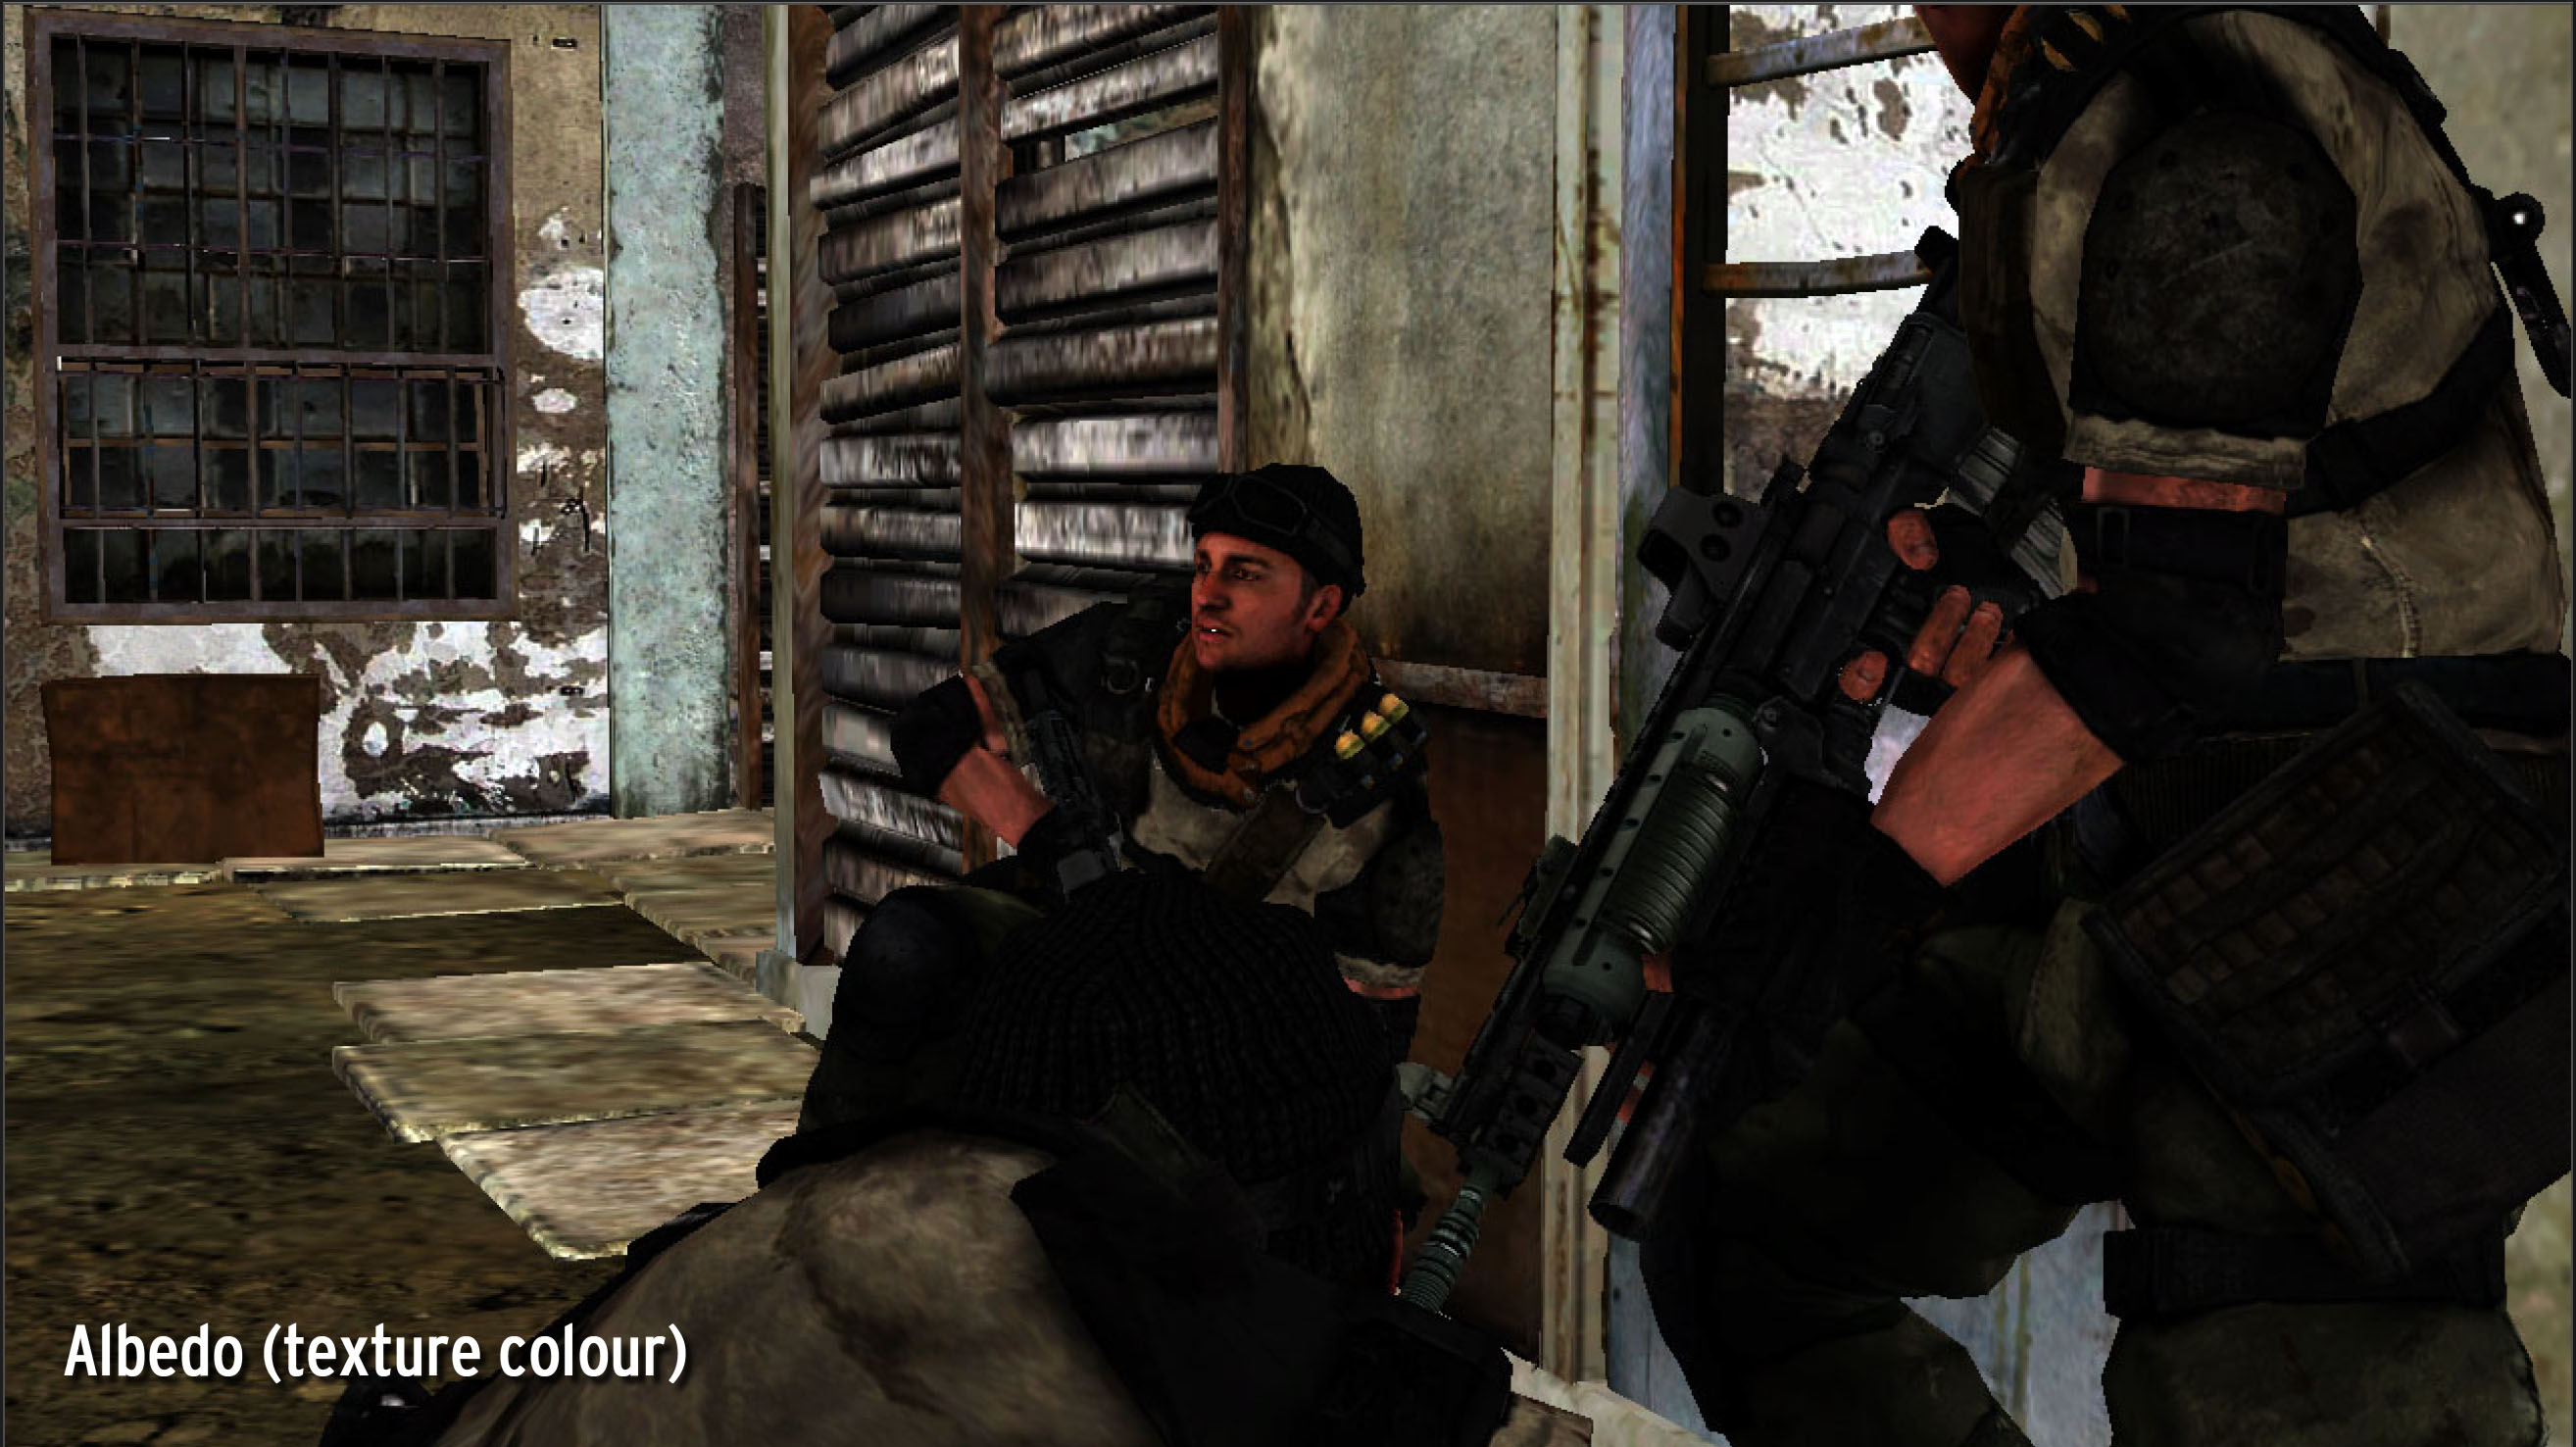
\includegraphics[width=175px]{images/graphics/killzone-2-buffer-albedo.jpg}
    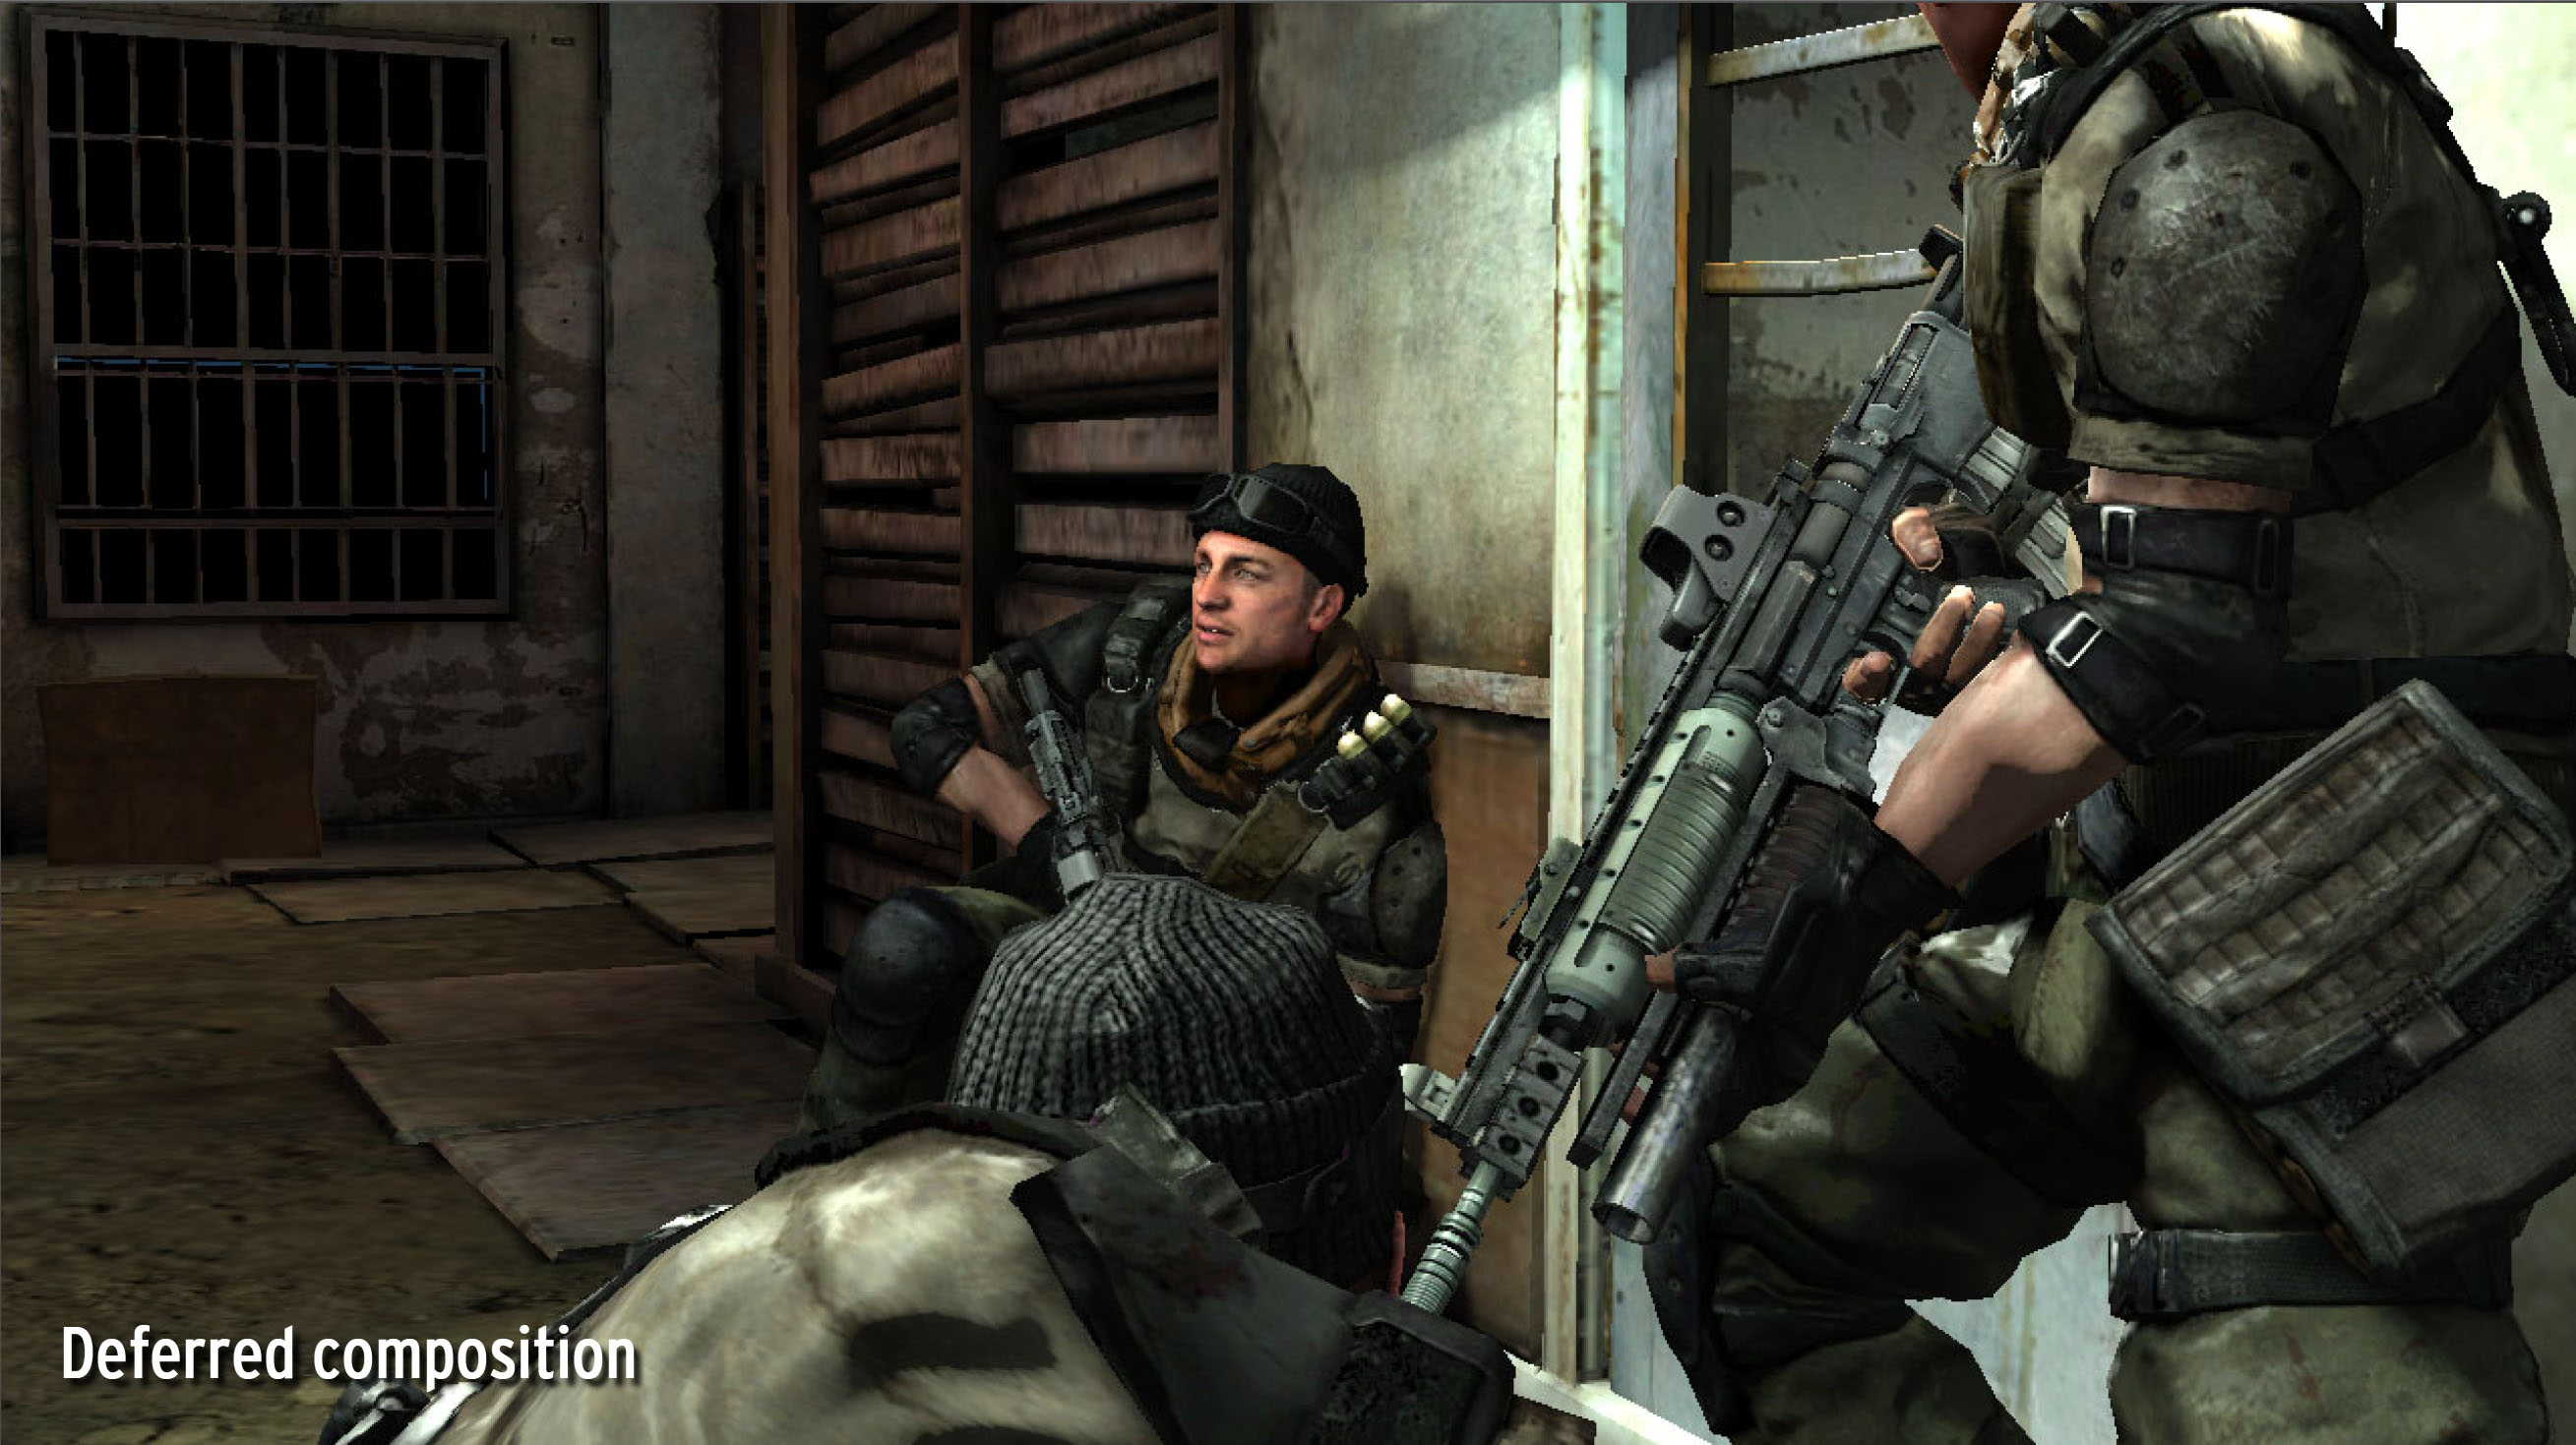
\includegraphics[width=175px]{images/graphics/killzone-2-buffer-composed-result.jpg}
    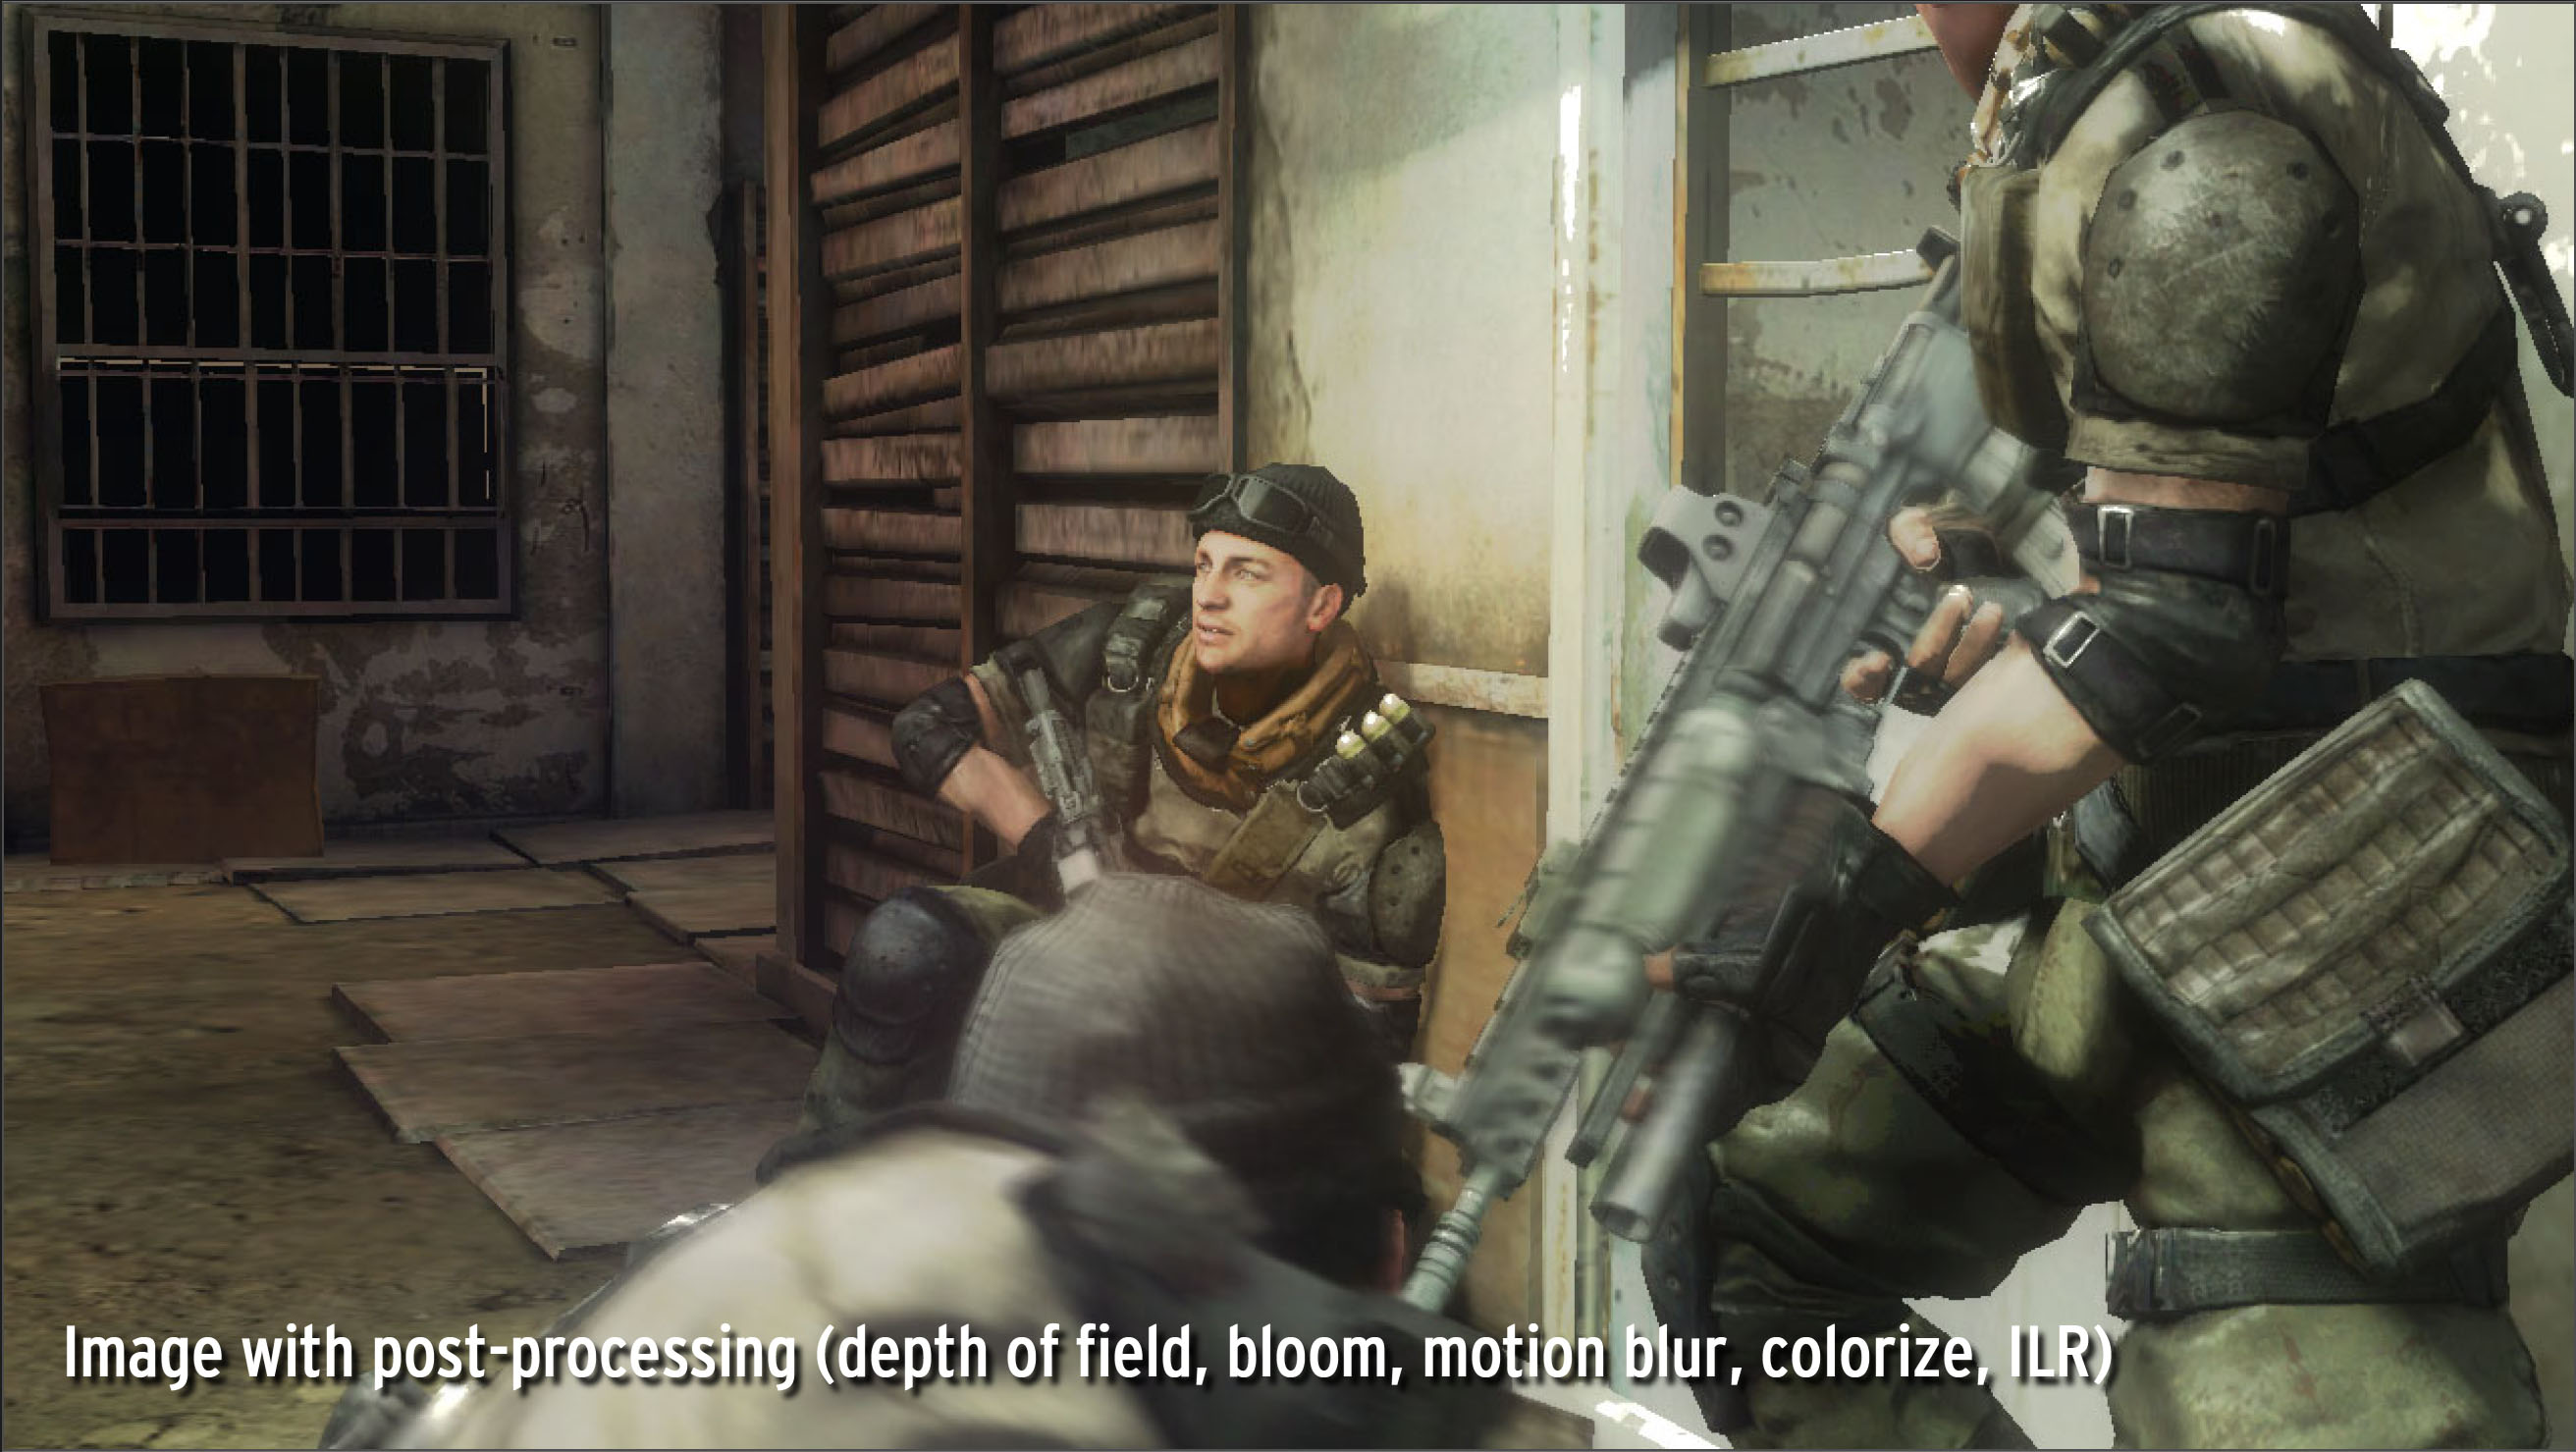
\includegraphics[width=175px]{images/graphics/killzone-2-buffer-post.jpg}
    \caption{Different buffers for \emph{Deferred Shading} in \emph{Guerilla Games'} \emph{Killzone 2} (2009) 
    \cite{Valient2007}.}
    \label{fig:deferred-shading-buffers}
\end{figure}

\noindent
As Akenine-Möller et al. point out, "the contribution of the models’ geometry has been fully decoupled from lighting 
computations" \cite{AkenineMoeller2018}. \emph{Deferred Shading} encompasses a lot more optimizations, like compression, 
light clustering, deferred texturing and more \cite{AkenineMoeller2018}. All these techniques combined can ultimately 
result in a more efficient shading model for specific use cases, for instance, when using a lot of lights in combination 
with high density geometry.\\

\noindent
The basic idea of \emph{Deferred Shading} influenced the next couple of years of real-time graphics technology and is 
still used today for state-of-the-art game development. Dispatching work for the \ac{GPU} to operate on and optimizing 
memory and data layouts for most efficient computation has also resulted in one of the latest trends in real-time 
rendering.

\subsection*{GPU Driven Rendering}

\begin{figure}[h]
    \centering
    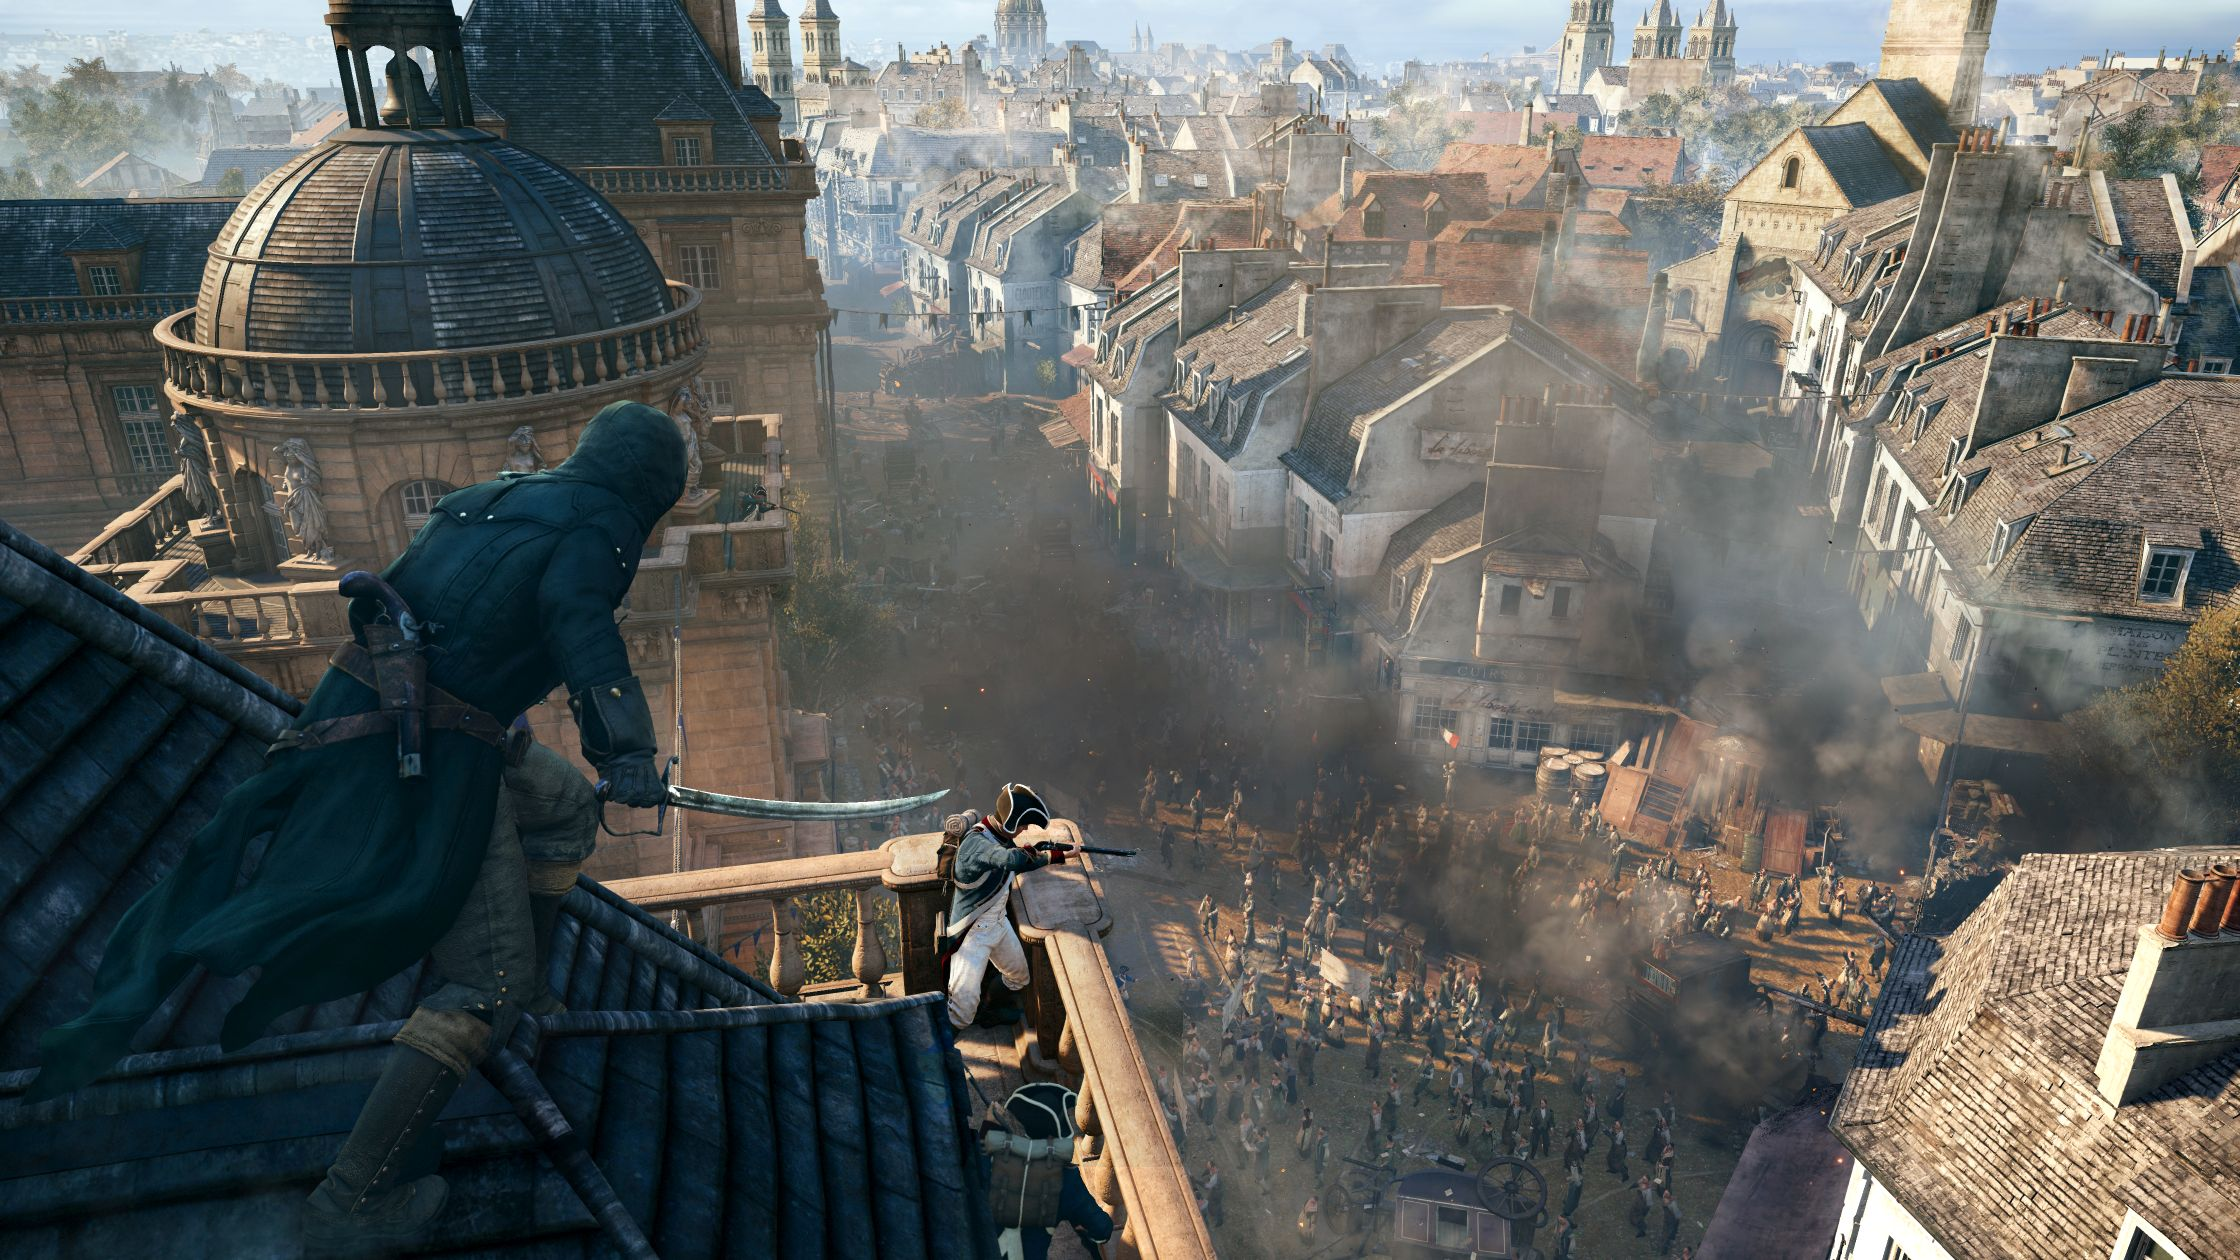
\includegraphics[width=300px]{images/graphics/assassins-creed-unity-gameplay.jpg}
    \caption{A screenshot of the game \emph{Assassin's Creed Unity} (\emph{Ubisoft} \cite{Ubisoft2014}, 2014) 
    showcasing the high density of geometry and far draw distances \cite{Burke2014}.}
    \label{fig:assassins-creed-unity-gameplay}
\end{figure}

\noindent [@TODO: Sources]
Over a decade after the first \ac{GPU} was introduced, hardware acceleration was the de facto standard in 
computer graphics and the rendering pipeline got more and more loaded with features, innovations and data. 
This led to a new bottleneck: The memory bandwith between the \ac{CPU} and \ac{GPU}. Soon, a new trend was 
developed: \emph{\ac{GPUDR}}. The goal of \ac{GPUDR} is, to minimize bandwidth between \ac{CPU} and \ac{GPU}. 
An ideal \ac{GPU} driven application would only update the camera related data (view and projection matrices) 
within a frame. Everything else would be computed by the \ac{GPU}. This trend arised with the rise of the 
\ac{GPGPU} and the better support for the more generalized \emph{compute shaders}. The defintion for when 
applications are \ac{GPU} driven and when not, is blurred, but one of the earlier games to make heavy use of 
\ac{GPUDR} is \emph{Assassin's Creed Unity} (\emph{Ubisoft} \cite{Ubisoft2014}, 2014), shown in figure 
\ref{fig:assassins-creed-unity-gameplay}. In 2015, Aaltonen et al. \cite{Aaltonen2015} held a presentation 
about \ac{GPUDR} on \emph{SIGGRAPH 2015}. This presentation pointed out previous work which was the basis for 
their approach, such as \cite{Greene93, Greene95, Hill11}. However, their approaches and innovations to 
computation of geometry, the use of \emph{occlusion culling} and \emph{deferred texturing} had a lasting impact 
on future games. \emph{Ubisoft's} technology allowed for a densly populated, dynamic, open world. Some of the 
technology used would only be seen in other games almost a decade later, when geometric computation was 
supported by specific hardware adaptions. Especially large, open games can profit from optimizations like storing 
scene data directly on the \ac{GPU}. In modern real-time computer graphics, the pre-computation by the \ac{CPU} 
and the data-transfer to the \ac{GPU} is replaced by data generation on the \ac{GPU} itself.

\subsection*{Mesh Shading Pipeline} \label{subsec-mesh-shading-pipeline}


\begin{figure}[h]
    \centering
    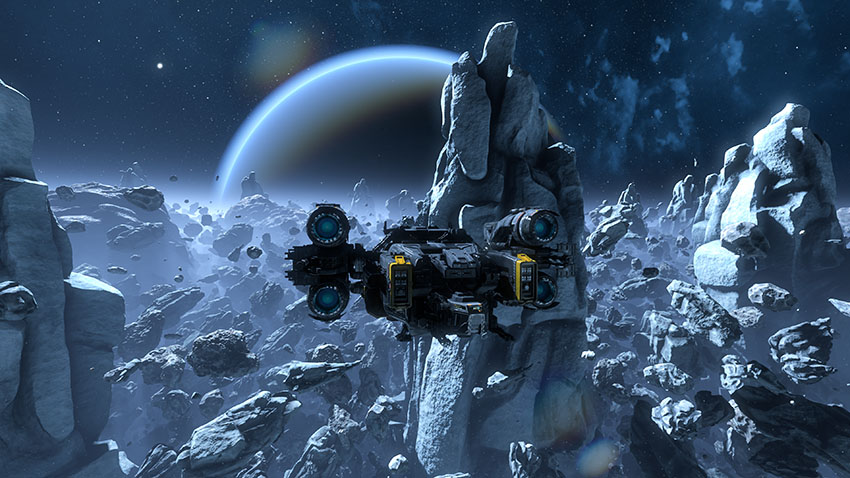
\includegraphics[width=300px]{images/graphics/mesh-shading-asteroids-demo.jpg}
    \caption{The offical \emph{Mesh Shading Pipeline} \emph{Asteroids} demo, featuring the new \emph{Mesh Shading Pipeline} (2018)
    and a high geometric density \cite{Kraemer2018}.}
    \label{fig:mesh-shading-asteroids-demo}
\end{figure}

\noindent
More elaborate algorithms for data computation on the \ac{GPU} led to a further increase in geometrical density.
This is why \emph{NVIDIA} introduced the new \emph{Mesh Shading Pipeline} in 2018 for \emph{NVIDIA Turing} \ac{GPU}s.
This pipeline improves the "old" vertex shader and features a more flexible way of computing and drawing geometry. 
It builds upon some of the innovations presented by Aaltonen et al.  \cite{Aaltonen2015} in 2015. Figure 
\ref{fig:mesh-shading-asteroids-demo} shows a frame of the initial demo provided by \emph{NVIDIA}. The new pipeline is 
discussed in more detail in chapter \ref{sec-mesh-shading} and are a central part of modern games such as \emph{Remedy's}
Alan Wake 2 (\emph{Remedy Entertainment} \cite{AlanWake22023}, 2023) or even \emph{Epic Games'} \emph{Unreal Engine 5} 
\cite{Karis2021}. 


\section{Motivation} \label{sec-motivation}

The latest innovations in computer graphics have been developing in different directions,
one of them being \ac{GPU} Driven Rendering. Minimizing dependencies between \ac{CPU} and \ac{GPU} 
has been an ongoing effort for the last decade. Many of the novel approaches which have been developed 
over the years are visible in the latest technology. But there are still plenty of use cases which are 
not yet living up to their full potential, considering modern hard- and software solutions.\\

\noindent 
One of those use cases is Voxel Rendering. Although there are ongoing efforts to improve voxel 
rendering performance, we believe that new innovations can be applied to this field of computer 
graphics. For years, voxel rendering has been using \ac{CPU} and \ac{GPU} optimization techniques 
in order to minimize the data computed by the \ac{GPU}. Many of these techniques refer to culling 
triangles or whole voxels. \ac{CPU} algorithms can make use of the regularity of the grid and 
reduce the amount of triangles sent over to the \ac{GPU}. [@TODO: Add sources for gpu acceleration 
in voxel rendering and write a bit more] \\

\noindent
This poses the question, if advanced culling techniques using modern, \ac{GPU} driven techniques can 
improve voxel rendering. An ideal culling would only draw visible voxels and ignore all other data 
not contributing to the visible and gameplay relevant scene. Therefore, our initial idea involved 
meshlet occlusion culling for large voxel scenes. The use of the new mesh shading pipeline in 
combination with efficient culling could drastically improve frame times. However, as will be 
pointed out in chapter \ref{subsubsec-two-pass-occlusion-culling}, for current occlusion culling 
algorithms to work, objects of different sizes are used to cull smaller instances or even meshlets.
Since voxels are always of the same size, this algorithm cannot be applied as is. Our approach 
relies on preprocessing data and applying approximations to the scene layout, so a variation of a 
common meshlet occlusion culling algorithm can be applied. In the next chapter 
\ref{cpt-technical-background} we first lay out a technical foundation before discussing related work 
in chapter \ref{cpt-related-work}. 
